% MSc Dissertation on pattern expression in Ovarian Cancer

\documentclass[tikz, 12pt,a4paper,oneside,fleqn]{article}

\usepackage[margin=1.5cm]{geometry}
\usepackage[utf8]{inputenc}
\usepackage{amsmath}
\usepackage{amsfonts}
\usepackage{amssymb}
\usepackage{fancyvrb}
\usepackage{setspace}
\usepackage{enumitem}
\setlist[description]{leftmargin=\parindent,labelindent=\parindent}

\usepackage{caption}
\captionsetup[figure]{labelfont=bf,format=hang,font={stretch=1.2, small}}
\captionsetup[table]{labelfont=bf,format=hang,font={stretch=1.2, small}}
\usepackage{graphicx}
\usepackage{rotating}
\usepackage{setspace}
\usepackage{afterpage}

\usepackage[linewidth=1pt]{mdframed}


\graphicspath{{/home/ipoole/Documents/gitrepos/MScDissertation/images/}}  % trailin '/' is required!
\newcommand{\plotspath}[1]{{/home/ipoole/Documents/gitrepos/HgsocTromics/Plots/#1}}

\definecolor{darkblue}{rgb}{0.0, 0.0, 0.55}
\usepackage{hyperref}
\hypersetup{
    colorlinks=true,
    linkcolor=darkblue,
    filecolor=blue,      
    urlcolor=darkblue,
}
\usepackage{subfig}
\usepackage{booktabs}  % Needed for pandas to_latex() output
\usetikzlibrary{positioning}


\newcommand{\etal}{{\em et al\/}}
\newcommand{\comment}[1]{\marginpar{{\tiny\singlespacing #1 \par}}}

\linespread{1.5}
% This sets Arial font (bit ugly!)
\usepackage{helvet}
\renewcommand{\familydefault}{\sfdefault}
\setlength{\parindent}{2em}
\setlength{\parskip}{1em}
\renewcommand{\baselinestretch}{1.5}

%\usepackage{titlesec}
%\titleformat{\subsubsection}
%   {\itshape\normalsize}{\thesubsubsection}{1em}{}

%%%%%%%%%%%%%%%%%%%%%%%%%%%%%%% SUBMISSION PAGE %%%%%%%%%%%%%%%%%%%%%%%%%%%%

\thispagestyle{empty}

\title{Disentangling patterns of gene expression in high grade serous ovarian cancer by matrix factorization}
\author{}

\begin{document}

%%%%%% Assesment Title Page
\begin{center}
\begin{center}

\includegraphics[scale=0.3]{images/UoE_SBO_logo.png}
\end{center}

\vspace{0.3in}

\begin{mdframed}
\begin{center}
\huge
\vspace{0.3in}
\bf
Disentangling patterns of gene expression in high grade serous ovarian cancer
\vspace{0.2in}
\end{center}
\vspace{0.2in}
\end{mdframed}

\vspace{0.3in}

\begin{mdframed}
\begin{center}
\large
\vspace{0.2in}
Student Exam Number: \bf{B156476}
\vspace{0.2in}
\end{center}
\end{mdframed}

\vspace{0.3in}

\begin{mdframed}
\begin{center}
\large
\vspace{0.2in}
In partial fulfilment of the requirement for the Degree of
Master of Science in Systems and Synthetic Biology at the
University of Edinburgh,
2019 / 2020
\vspace{0.2in}
\end{center}
\end{mdframed}

\vspace{0.3in}

\begin{mdframed}
\begin{center}
\large
\vspace{0.2in}

Disssertation Supervisor:  Dr. Ailith Ewing
\vspace{0.2in}
\end{center}
\end{mdframed}
\end{center}

\newpage
\setcounter{page}{1}
%\pagestyle{headings}

\tableofcontents

\newpage

%%%%%%%%%%%%%%%%%%%%%%%%%%% Start of report for real %%%%%%%%%%%%%%%%%%%

\begin{abstract}
Here is the abstract
\end{abstract}
\newpage


\section{Introduction}

\subsection{Epithelial Ovarian Cancer}
\label{sec-epithelial-ovarian-cancer}


Ovarian cancer (OC) is a heterogeneous disease, presenting with a wide range of pathologies and molecular characteristics .  The World Health Organisation sets out five subtypes of epithelial ovarian carcinomas (EOC) grouped into two main types\cite{Kossai2018, Lisio2019}: 

\begin{description}
\item[Type I] are low grade with generally good prognosis, with two subtypes:
\begin{description}
\item[Low grade serous] affecting the epithelial membrane which secretes serous fluid), $< 5$\% of cases
\item[Mucosal] affecting membrane rich mucous glands, 2 - 3\% 
\item[Clear cell] relating to the presence of clear cells in histology, 5 - 10\%.
\end{description}
\item[Type II] are more aggressive (rapidly growing), typically carrying P53 mutations with defects in mechanisms of DNA repair. Three subtypes:
\begin{description}
\item[Endometrial] affecting the the inner lining of the uterus, 10 \% of cases.
\item[\emph{High grade serous OC (HGSOC)}] affects the epithelium of the ovaries and fallopian tubes.  It is the most common type of OC, accounting for 70\% of cases, and most serious of the OC subtypes and the focus of this dissertation.
\end{description}
\end{description}

HGSOC typically occurs in older patients and is diagnosed at a late stage.   Histology of HGSOC is similar to the low grade subtype, but the cancer develops along distinct molecular pathways. 

Treatment options for HGSOC depend on tumour stage and include surgery (tumour debulking) or platinum-based chemotherapy (e.g. Cisplatin).  Acquired resistance to platinum is a major cause of disease recurrance\cite{Patch2015} and so motivates research into the genomic events which lead to such resistance.


\subsection{Patterns of gene expression in HGSOC}

Identifying the patterns -- or ``signatures'' -- of gene expression has been an active research area, for the purposes of understanding the carcinogenesis pathway, subtype classification, predicting survival prognosis, predicting treatment response and understanding the causative mechanism of risk factors; there is much cross-over between these areas, however.

\subsubsection{Carcinogenesis pathways including homologous repair deficiency}

BRCA1 inactivation is known to cause chromosomal instability in many cancers.  Pradhan \etal\ \cite{Pradhan2010} investigated the role of BRCA1 in HGSOC by copy number and expression analysis, finding surprisingly that inactivation has no relationship with gross genomic alteration.  They leave open the question whether DNA repair by PARP plays a role.   The relationship between BRCA1/2 and DNA repair -- specifically homologous repair deficiency (HRD) -- is picked up by Ewing \etal \cite{Ewing2020}.  They study the complex interplay of single nucleotide variants and large structural variants as they impact BRCA1/2 disruption and thence HRD.  This work suggests that when BRCA1/2 loss is detected in HGSOC patients, there may be a clinical role for PARP inhibitors, since this would prevent error-prone non-homologous repair by PARP, and so selectively kill BRCA1/2 disrupted cells.

Studying the combined landscape of chromosomal rearrangements, driver mutations (particularly TP53, BRCA1/2), methylation and gene expression profiles has lead to a better understanding of the molecular events involved in the progression HGSOC and the development of chemoresistance \cite{Patch2015}.  The sequence of events is complex, however, and not easily summarised here.   A similar integrative / multiplatform approach is taken in \cite{He2017a} and \cite{Hoadley2014}.

\subsubsection{Subtype classification}
\label{sec-subtype-classification}

A relatively early (2003) expression microarray based work demonstrated clustering into lymphocyte related genes (IGH3, IGKC, IGLJ3), extracellular matrix/stromal related (COL11A1, COL3A1, MMP2, SPARC, RBBP1) and six other clusters \cite{Schaner2003}.

A relatively early (2003) expression microarray based work demonstrated clustering into lymphocyte related genes (IGH3, IGKC, IGLJ3), extracellular matrix/stromal related (COL11A1, COL3A1, MMP2, SPARC, RBBP1) and six other clusters \cite{Schaner2003}.

Wang \etal\ \cite{Wang2017c} use NMF clustering (see section \ref{sec-nmf}) to identify five subtypes of HGSOC informative of outcomes: 1:mesenchymal, 2:immunoreactive, 3:proliferative, 4:differentiated and 5:anti-mesenchymal.
Subtypes 2 and 5 are found to be associated with better survival.

Disruption of the PI3K-AKT signalling pathway is known to be significant in several cancers, due to its role in regulating apoptosis.  
Espinosa \etal\ \cite{Espinosa2011} used unsupervised clustering techniques to investigate expression of 22 genes of this pathway.  
They found that HGSOC cases formed two separate clusters; the cluster with high expression of CASP3, XIAP, NFKB1, FAS and GSK3B was linked with better outcomes.

An integrative network approach has identified two distinct subtypes of ovarian cancer, distinguished by differences in expression of genes related to transcription factors which influence angiogenesis \cite{Glass2015}.  The authors suggest that the regulatory networks highlighted by their analysis can lead to targetting with specific drugs.

A recent pre-publication develops a pipeline for sub-type prediction with the potential to be used clinically \cite{Talhouk2020}.
The NanoString gene expression platform is used.  Their strategy was to focus on small set of 513 genes (vs $\sim$21,000 protein coding genes) known from the literature to have relevance to subtyping.
Two approaches were followed by different teams.  ``All Array": used expression array data from 1650 patients across 14 studies evaluating 9 supervised learning algorithms by bootstrap, selecting an AdaBoost -like method. The ``TCGA" team used 434 patients from The Cancer Genome Atlas (TCGA\footnote{I'm always amused by the genetics pun in the naming of this resource!}) evaluating 5 algorithms by cross-validation selecting a random forest.  "All Array" had the advantage of more data but needed attention to batch effects. A final classifier took a consensus of the two methods based on a minimal gene set (order 40 of genes), validated by a leave-one-out (patient level) approach.  Survival analysis was carried out stratified by predicted subtype.

\subsubsection{Treatment response and survival}

As we have seen in section \ref{sec-epithelial-ovarian-cancer}, EOC subtypes are closely linked with survival, never-the-less much research is directed at finding direct links with expression.

The prognostic value of expression signatures is demonstrated by the ``Classification of Ovarian Cancer" (CLOVAR) system \cite{Verhaak2013}.  
Single-sample gene set enrichment analysis (ssGSEA) is used to obtain scores for previously reported expression signatures: differentiated, immunoreative, mesenchymal and proliferative.  
An outcome prediction model based on these signatures gave good survival stratification (likelihood ratio 10.8 between above/below median groups) on a validation dataset) which improved to 15.7 when augmented with BRCA1/2 mutation status and other post-operative clinical factors.

An explicit supervised learning approach can be taken, as in Berchuck \etal, where a hybrid decision tree plus linear discriminant model demonstrated survival stratification in both cross-validation and external validation experiments, based on microarray expression data.   
They found expression of CSFT3, ABCD3, MAL and APMCF1 to be the most influential; in fact the decision tree was almost entirely driven by the first two of these

Mairinger \etal\ screened 770 immune related genes to identify 11 differentially expressed genes associated with response to platinum treatment.  
They find that expression of HS11B1, DNBT1, CKLF, NUP107. CCL18, LY96, ATG7, SLAMF7, CXCL9 is associated with better survival, while IKBKG and SDHA associate with with poor survival.

The platinum based drug Cisplatin is a key treatment in ovarian cancer, yet tumours often develop resistance, possibly related to the host's immune response.  
Understanding and predicting such resistance is therefore of clinical importance and is addressed by Maringer \etal\ \cite{Mairinger2019} through expression analysis using the NanoString platform with a panel of 770 immune related genes.   
They find the following genes to be significantly related to platinum resistance: KLRC1, TCF7, CD274, HSD11B1, COLEC12, PDGFC, FCF1, BMI1, TNFRSF9, ATG10, EWSR1.

Finding a clear, robust correlation between gene expression patterns and survival is not straight forward.  
One substantial meta-analysis applied 16 previously published gene sets to two studies from GEO (199 samples) which included survival information, and found no significant predictive power \cite{Fekete2012}.  
Although, within the same study, the authors did identify predictive genes, in particular SNGC, MAPT, ESR2 and PGR.

Expression of a single gene -- CD38, which codes for a transmembrane glycoprotein -- has recently been shown to have survival prognostic value on its own \cite{Zhu2020}.
CD38 has a role in the breakdown of nicotinamide adenine dinucleotide ($\mbox{NAD}^+$), and is also a cell marker of lymphocytes.
CD38 is over expressed in myloma cells, thence its importance as a prognostic marker and a potential drug treatment target.  
It is worth mentioning that the analysis in this paper made use of the Gene Expression Profiling Interactive Analysis (GEPIA) database, which conveniently supports survival analysis with respect of any given gene, against a range of TCGA gene expression databases.

\subsubsection{Association with other risk factors}

Obesity has been shown to negatively impact prognosis in ovarian cancer, possibly through difficulties in matching chemotherapy dose with patient BMI  \cite{Au-Yeung2014}.  A more direct molecular link is proposed by Cuello \etal\ \cite{Cuello2018}.  They used NMF based clustering to demonstrate that expression of genes linked with obesity and lipid metabolism impart poorer progression free survival, independent of known HGSOC driver gene expression.  The link is complex however, there been many confounding non-molecular based reasons for a link between high BMI and HGSOC survival, including later diagnosis and compromised operability.  Some studies (e.g. \cite{Hew2013}) conclude no overall link at all.



%Stratification of HGSOC by immunohistochemistry is addresses Kamble \etal. \cite{Kamble2019}.  They identify a panel of six biomarkers -- TCF21, E-cadherin, PARP1, Slug and AnnexinA2.   These markers allow stratification into categories including Mesenchymal-to-epithelial transition, Homologous recombination repair and Epithelial-to-mesenchymal transition.  This, they argue, allows selection of class-specific inhibitor drugs such as Olaparib and Rucaparib.

\subsection{Matrix factorization for dimensionality reduction}
\label{sec-matrix-factorization-intro}

Dimensionality reduction concerns representing high dimensional data in far fewer dimensions, with minimal loss of information.  This is possible in many cases because dimensions -- or equivalently elements of a feature vector -- are highly correlated.  In the case of gene expression analysis, the dimensionality is of the order 20,000, i.e. the number of transcripts (mRMA transcribed genes) being considered.  However, it is known that sets of genes act in concert, their expression thus being correlated, so reducing the true degrees of freedom in the data.  The challenge is to uncover these true degrees of freedom, which constitute our ``patterns of gene expression''.

The three matrix factorization methods considered in this work are described below.  All are forms of dimensionality reduction, but have differing criteria they aim to optimise.  The number of target dimensions (or components, factors, metagenes -- these terms are used somewhat synonymously) is referred to as the rank, $k$.
\subsubsection{Non-negative matrix factorization (NMF)}
\label{sec-nmf}
As the name implies, this is only applicable to matrices with +ve or zero elements, and finds components which are themselves +ve or zero.   This property make the resulting factorization more interpretable since the components are strictly additive.   
NMF has been applied widely in -omics research, originally to gene expression microarrays  and latterly to RNA-seq datasets.  
A particular value of NMF is that it allows for input samples to be directly assigned to one of $k$ clusters.   
The optimization function on which NMF is based can be tuned to achieve a \emph{sparse} factorization result, that is one in which only a small number of elements in the achieved factorization are non-zero, a property which further simplifies interpretation.
\cite{Brunet2004}.
%
\subsubsection{Independent component analysis (ICA)} 
The goal of ICA is to represent the given matrix with components which are statistically independent of each other.  It was originally proposed to solve the blind source separation problems \cite{Comon1994}. If the input matrix of samples were drawn from a multivariate Gaussian distribution, then the result would be no different to that of PCA.    Where the data is non-Gaussian however, ICA results in components which separate out independent sources of variation.  See \cite{Sompairac2019} for a full explanation, from which figure \ref{fig-pca-ica-nmp-explanation} is taken.
\subsubsection{Principal component analysis (PCA)}
PCA is a well known technique for dimensionality reduction, based on eigenvalue decomposition.  It is arguably the ideal, efficient solution for data which is multivariate Gaussian distributed -- or can assumed to be so.  PCA results in components which are ordered by the proportion of total variance they explain, and are mutually orthogonal.

The contrasting results of the three methods is illustrated in figure \ref{fig-pca-ica-nmp-explanation}. \emph{TODO: add explanation of this diagram}

\begin{figure}[ht]
\begin{center}
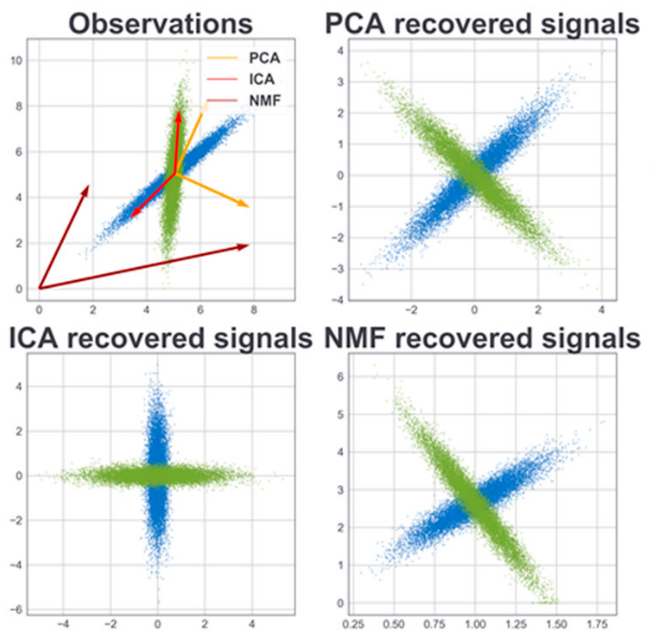
\includegraphics[scale=0.4]{Sompairac_ICA_NMF_PCA.png}
\end{center}
\caption{Illustrating the differing results of component extraction by PCA, ICA and NMF.  From \cite{Sompairac2019}}
\label{fig-pca-ica-nmp-explanation}
\end{figure}


Conventionally, transcriptomics expression arrays are oriented with genes (or transcripts) as rows, and samples (e.g. patients) in columns.   
A typical expression array might have in the order of tens of thousands of rows and hundreds of columns.  
MF methods reduces this large $M \times N$ (genes $\times$ samples) matrix into two smaller matrices.
In the general terminology of Stein-O'Brien \etal\ these are the $M \times K$ \emph{pattern matrix} and the $K \times N$ \emph{amplitude matrix}.  $K$ (or $k$ as we will use) is typically small of the order 10, and refers to the number of extracted \emph{factors} (or components); it is the rank of the factorization.
Since we are focussing on transriptomics, rather than pattern and amplitude we will use the terms \emph{metagenes} and \emph{metasamples} respectively, which are in common useage.  The symbol conventions for these matrices varies depending whether NMF, ICA or PCA is being discussed.   NMF generally uses $W$ and $H$ respectively while ICA generally uses $S$ and $A$.  PCA tends to be differently formulated, but $W$ and $T$ sometimes used.   The original matrix to be factorized is variously named $X$ or $V$.

In this work I wish to treat and discuss the three factorization methods in a unified way.  Thus, for the remainder of this dissertation the following notational conventions are adopted:
\begin{description}
\item[Expression matrix:] $X$ $(M \times N)$
\item[Metagene matrix:] $W$ $(M \times K)$
\item[Metasample matrix:] $H$ $(K \times N)$
\end{description}
where $N$ is the number of patients (or samples), $M$ is the number of genes and $K$ is the factorization rank, i.e. the number of components or factors.  Thus the factorization is written
\begin{equation}
X \approx W H
\end{equation}
Adding subscripts to indicate the row,column orientation of the matrices:
\begin{equation}
X_{M,N} \approx W_{M,K} H_{K,N}
\end{equation}
as illustrated in figure \ref{fig-matrix-factorization} (a).

\begin{figure}[ht]
\def\M{2.2cm}
\def\N{1.3cm}
\def\K{0.3cm}
\def\fudge{-0.8mm}
\centering
\subfloat[Optimising independence of Meta\underline{genes}]{
\begin{tikzpicture}[node distance = 0.25cm]
	\node (X) [draw, fill=green, minimum height=\M, minimum width=\N] {\large X};
	\node [right=of X] (eq) {\large $\approx$};
	\node [right=of eq] (S) [draw, fill=yellow, minimum width=\K, minimum height=\M] {\large W};
	\node [right=of S] (times) {\LARGE$\times$};
	\node [right=of times] (A) [draw, fill=cyan, minimum width=\N, minimum height=\K] {\large H};
	
	\node [below=\fudge of X] {\tiny{$N$ Samples}};
	\node [left=\fudge of X] {\rotatebox{90}{\tiny{$M$ Genes}}};
	\node [below=of X, text width=2cm, align=center] {\small Expression matrix};
	
	\node [below=\fudge of S] {\tiny{$K$ Metagenes}};
	\node [left=\fudge of S] {\rotatebox{90}{\tiny{$M$ Genes}}};
	\node [below=of S, text width=2cm, align=center] {\small Metagenes};
	
	\node [below=\fudge of A] {\tiny{$N$ Samples}};
	\node [left=\fudge of A] {\tiny{$K$}};
	\node [below=of A, text width=2.5cm, align=center] {\small Metasamples};
\end{tikzpicture}} 

\subfloat[Optimising independence of Meta\underline{samples}]{
\begin{tikzpicture}[node distance = 0.25cm]
	\node (X) [draw, fill=green, minimum height=\N, minimum width=\M] {\large X};
	\node [right=of X] (eq) {\large $\approx$};
	\node [right=of eq] (S) [draw, fill=cyan, minimum width=\K, minimum height=\N]{\large W};
	\node [right=of S] (times) {\LARGE$\times$};
	\node [right=of times] (A) [draw, fill=yellow, minimum width=\M, minimum height=\K]{\large H};
	
	\node [below=\fudge of X] {\tiny{$M$ Genes}};
	\node [left=\fudge of X] {\rotatebox{90}{\tiny{$N$ Samples}}};
	\node [below=of X, text width=2cm, align=center] {\small Expression matrix};
	
	\node [below=\fudge of S] {\tiny{$K$ Metasamples}};
	\node [left=\fudge of S] {\rotatebox{90}{\tiny{$N$ Samples}}};
	\node [below=of S, text width=2.5cm, align=center] {\small Metasamples};
	
	\node [below=\fudge of A] {\tiny{$M$ Genes}};
	\node [left=\fudge of A] {\tiny{$K$}};
	\node [below=of A, text width=2cm, align=center] {\small Metagenes};
\end{tikzpicture}}
\caption{Two ways of configuring matrix factorization in the context of gene expression analysis.
In configuration (a) NMF and ICA will optimise the \emph{metagenes}, while in (b) the \emph{metasamples} are optimised. }
\label{fig-matrix-factorization}
\end{figure}

In the case of NMF and ICA, the $W$ and $H$ matrices cannot be trivially exchanged and transposed.  This is because the optimisations (sparsity and independence respectively) which define these algorithms are focussed on the $W$ matrix.  It is perfectly possible to apply these algorithms to gene expression analysis with exchanged and transposed meanings of $W$ and $H$, and this is illustrated in figure \ref{fig-matrix-factorization} (b).  In this case it is the properties of the \emph{metasamples} which will be optimised.  Thus, the two forms are different in substance, not simply in notational convention.

There is substantial confusion and lack of clarity in the way that matrix factorization, particularly ICA, is applied in transcriptomics research.  
``Surprisingly, both ways of applying ICA to omics data are wide-spread, and sometimes it takes an effort to figure out in which way ICA was applied" \cite{Sompairac2019}, and ``Different protocols to apply ICA to transcriptomic data exist and currently no single standard approach has been defined. The main difference in the existing approaches consists in what is considered as source signal matrix in the decomposition" \cite{Cantini2019}.  
According to Cantini \etal\, references \cite{Au-Yeung2014}, \cite{Kairov2017}, \cite{Kong2008} and \cite{Lee2003} optimise metagenes, while references \cite{Meng2016} and \cite{Barillot2013} optimises metasamples.


\subsubsection{Determining the optimum number of factors}

The number of factors, or rank $k$, to extract is a key decision in any matrix factorization approach.  In this regard, PCA differs from ICA and NMF.  In PCA it is reasonable to extract all factors, setting $k=N$, the factors being ranked by the associated eigenvalue which also ranks the proportion of variance explained.   However, that approach is not valid for ICA and NMF, since differing sets of factors will be obtained for different $k$, and for a given choice of $k$ all factors are equally important -- they do not rank \cite{Stein-OBrien2018}.

The problem of determining the optimal $k$ for a given expression matrix is addressed  by Kairov \etal\ \cite{Kairov2017}, based on optimizing the \emph{stability} of the components over multiple algorithm initializations.


\subsection{Research goals}
This work is concerned with analysing the patterns gene expression in HGSOC by dimensionality reduction techniques of matrix factorization, and relating these patterns to clinical and genomic features.

The following research questions were set out early in the project. \emph{TODO: tweak these goals!}
\begin{enumerate}
\item Which are the influential genes in HGSOC according to gene expression data?   Do these confirm published results?
\item Which of PCA, ICA and NMF is best suited to this analysis?
\item For identified genes, what is the underlying biology?
\item Can we discriminate subtypes of HGSOC from expression data?
\item Is there value in incorporating somatic and germline genomic data?
\end{enumerate}

%%%%%%%%%%%%%%% METHODOLOGY %%%%%%%%%%%%%%%%%

\section{Methodology}

\subsection{Outline}

Our overall approach is to use \emph{unsupervised} machine learning methods to represent gene expression data in a small number of features, then to study whether these features correlate with clinical and biological variables.  This is appropriate in our case, since of the two datasets available (described below), one (TCGA) has relatively large n but little available metadata, while the other (AOCS) is much smaller but has more useful metadata of genomic features.   This motivates an approach of unsupervised learning on the TCGA dataset which is then transferred to the AOCS dataset.

\subsubsection{Datasets}
Two gene expression datasets were assailable for this work (n refers to number of patients, g refers to number of genes).
\begin{enumerate}
\item The Cancer Genome Atlas (TCGA) derived, n=274, g=19,601, with metadata on survival
\item Austrailian Ovarian Cancer Study (AOCS) \cite{Patch2015}, n=80, g=19,730, with metadata on survival, cellularity and additional genomic features. Several of the studies reviewed earlier also use data from the Australian Ovarian Cancer Study (AOCS): \cite{Patch2015,Ewing2020,Cuello2018,Au-Yeung2014}.
\end{enumerate}
TODO: \emph{more explanation of the provenance of these datasets}.

Expression data for the AOCS and TCGA datasets was received for this project in a spreadsheet format, having been derived from the RNA-Seq data as described in \cite{Ewing2020}, including  normalization by variance stabilizing transformation.   


\subsubsection{Method outline}
An overview of the methodology adopted in this work is shown in figure \ref{fig-method-overview}, consisting of:

\begin{figure}[ht]
\begin{center}
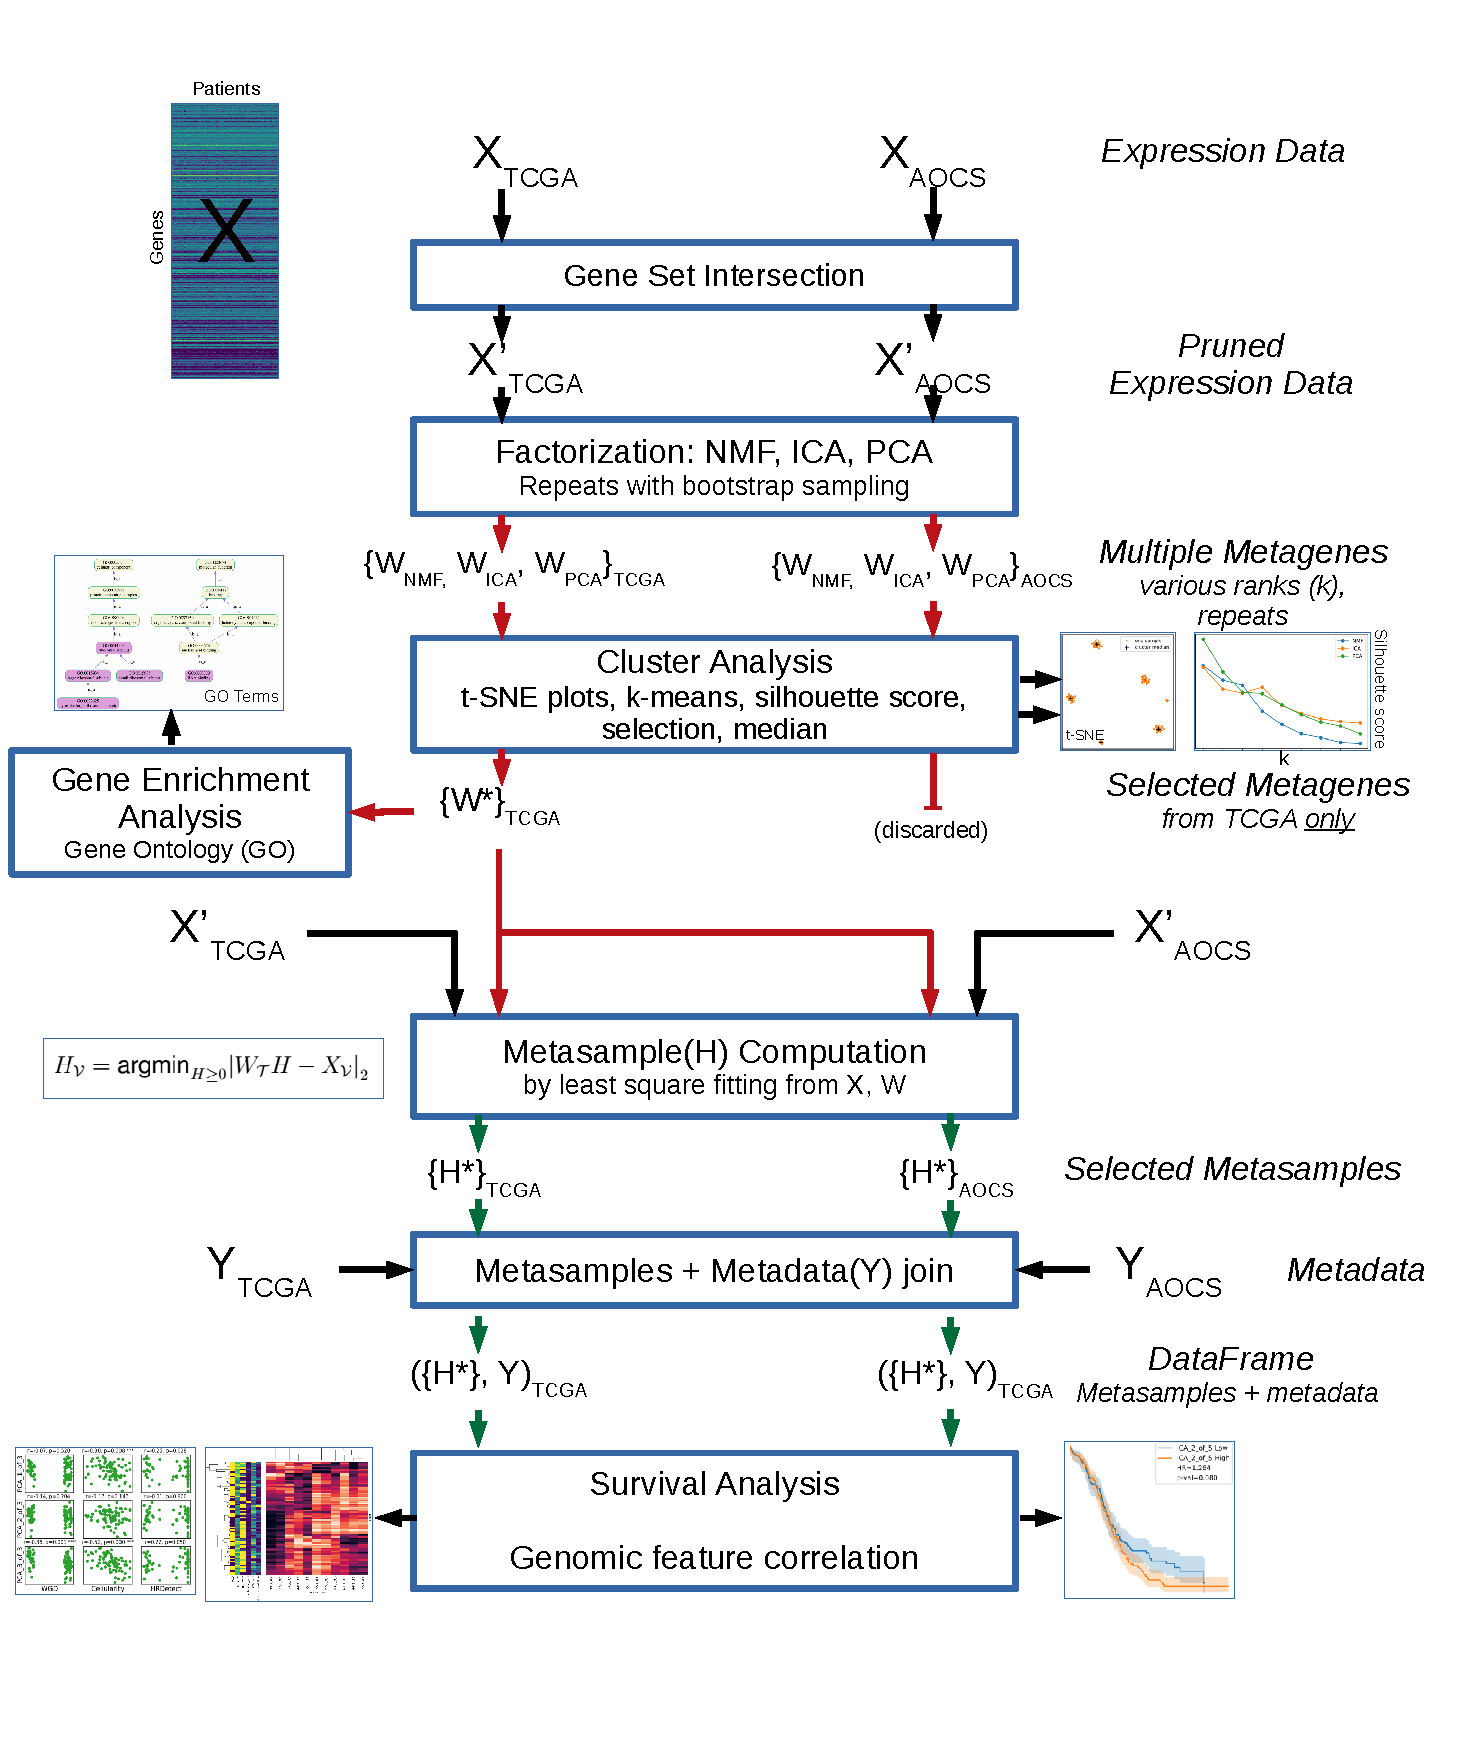
\includegraphics[scale=0.7]{methodlology_overview.pdf}
\end{center}
\caption{Overview of methodology as information flow.  The diagramatic convention here is that at each stage, both datasets -- TCGA and AOCS -- are processed separately by the given algorithm.  The exception is Gene Set Intersection, which involves interaction between the datasets.}
\label{fig-method-overview}
\end{figure}

\begin{enumerate}
\item
Identification of a consistent gene set between the TCGA and AOCS datasets.
\item
Unsupervised metagene extraction by matrix factorization methods : NMF, ICA and PCA.
\item
Metagene selection for robustness by k-means clustering of bootstrap resampled factorizations evaluated by silhouette score, based on the TCGA dataset.
\item
Investigation of biological significance of determined factors by gene enrichment analysis against the Gene Ontology (GO).
\item
Computation by least squares optimisation of metasamples associated with with each TCGA derived metagene against TCGA and AOCS datasets.
\item
Alignment of available metadata with computed metasamples, for TCGA and AOCS.
\item 
Survival analysis on TCGA and AOCS to investigate relationship between metasamples and patient survival.
\item
Scatter plots and heat maps to investigate the relationships between metasamples and genomic features available for the AOCS dataset.
\end{enumerate}

\clearpage

\subsubsection{Tools}
\begin{itemize}
\item Python 3.6
\item PyCharm Integrated Development Environment
\item Numpy for high performance matrix manipulation
\item Pandas for data frame handing
\item Matplotlib and Seaborn for general plotting
\item Scikit-learn for matrix factorization and k-means clustering
\item GOATOOLS package for gene enrichment analysis against GO
\item Lifelines package for survival analysis.
\end{itemize}

A full list of software and libraries used, with versions, is given in appendix \ref{sec-software-versions}.



\subsection{Gene set intersection}
\label{sec:gene-set-intersection}

In order to allow factorizations found in the TCGA dataset to be applied to the AOCS dataset it is necessary (or at least convenient) to synchronize the set of genes over which the expression matrices are defined.   As provided to this project, the TCGA and AOCS datasets cover 19,610 and 19,730 protein coding genes respectively, 19,566 of which are common to both (according to ENSG encodings).  Thus, both datasets were pruned to the 19,566 intersection set and ordered consistently.

\subsection{Matrix factorization computation}
One of the aims of this work is to compare the efficacy of three methods of dimensionality reduction -- NMF, ICA and PCA -- as explained in the introduction.   
%The three methods have different properties and notational conventions, but to simplify the discussion here we adopt the notation $X \approx W H$ for all three methods, where $X$ is the (genes, patients) expression matrix  $W$ is the (genes, factors) metagenes matrix and $H$ is the (factors, patients) metasamples matrix.   

Some of the key algorithm hyper parameters of each method were investigated and tuned with respect to reconstruction accuracy, specifically the root-mean square (RMS) difference between $X$ and $W H$. The following parameters were explored in each case:
\begin{description}
\item[NMF:] Parameters {\tt max\_iter} (algorithm iterations) and {\tt tol} (tolerance of convergence) were optimised for good accuracy and acceptable execution time.  Other parameters of interest are {\tt alpha} (multipluer for regulation term) and {\tt l1\_ratio} (multiplier for L1 regularization, when {\tt alpha} $> 0$).  L1 regularization  favours elements being precisely zero, whereas L2 regularization will encourage them to be small.  These parameters have not been explored in this project, and the default {\tt alpha = 0} (no regularization) was used.
\item[ICA:]  Parameters {\tt max\_iter} and {\tt tol} were investigated as for NMF above.  Additionally, options for the entropy functional which forms the basis of the optimiziation were investigated.
\item[PCA:] This is in principle a deterministic algorithm based on eigenvector decomposition.  However, {\tt sklearn.decomposition.PCA} uses a more efficient 'randomized' algorithm when the given matrix is larger than 500 in both dimensions.  Thus in our use case PCA is seen to have stochastic behaviour.
\end{description}

\emph{TODO: probably best to state the chosen hyper parameters here}

\subsection{Metagene selection by cluster coherence}
\label{sec-metagene-selection}
Deciding on the number of components (factors, metagenes) to extract -- that is the factorization rank -- is key.  Taking more components results in more accurate representation of the observed expression matrix and provides more avenues to explore the underlying biology.  However, it is important that the metagenes are \emph{stable}, that is that they have reliable meaning when transfered to other datasets.   There are two sources of variation or instability to consider.

Firstly, NMF and ICA are inherently stochastic algorithms, sensitive to their starting state, so repeated runs give different results.

A second and more fundamental source of variation of relevance to all three factorization methods is \emph{sampling error}.   Our factorizations are based on a small ($N=80$ or $N=374$) sample of patients drawn from the population of HGSOC patients; our particular datasets are just two examples of many different `draws' which could have been made from that population.

\emph{Bootstrap sampling} (also know as \emph{Monte Carlo} simulation) is a common method of empirically propagating the consequence of sampling error when the distribution or processing operations are difficult to model mathematically.   This is implemented by performing factorizations multiple times, at each iterations choosing N samples from the N available \emph{with replacement}.   For this work 50 repeats were performed, being a compromise between achieving an adequate simulation without overly burdensome computation time.  The overall process is summarised as pseudocode in figure \ref{fig-clustering-psuedocode}.  

A complication arises in the computation of ICA and PCA facorizations, in that essentially the same factor can arise as $w$ or $-w$ -- i.e. $180^\circ$ rotated vectors. These would appear as separate cluster in repeated sampling, and confound attempts to collect and aggregate.  The solution adopted here is to normalise each factor by requiring that the most extreme element -- i.e. having the greatest absolute value -- is positive, the whole factor being negated if this is not the case.  This is arguably over simplistic, but seems to be effective in practice.

Each of the three factorizer methods was evaluated for rank $k$ between 2 and 10.  In each case, 50 iterations of factorization are performed on bootstrap samples, generating $50 k$ instances of 19,566 dimensioned metagenes.  Two dimensional t-SNE plots were generated for visualization purposes.   If sampling and algorithm initialisation error are modest then we expect to see $k$ tight clusters of points.   To avoid lengthy computation in the t-SNE clustering, the metagenes were first reduced to $r=20$ dimensions by PCA; brief experiments showed that this reduction had negligible effect on the t-SNE visualisation for $r \geq 10$.   

In order to obtain median estimates of the $k$ metagenes from the $50 k$ which were generated, k-means clustering was performed in the PCA reduced ($r=20$ dimension) space, delivering $k$ sets of points.  These were referenced back to the original 19,566 dimensioned metagenes and the per-dimension median calculated.  These $k$ median metagenes were saved to a file named for the specific factorizer and rank $k$.  

The k-means clustering further allowed for a quantitative assessment of cluster coherence for the particular choice of factorizer and rank, via the \emph{silhouette score}.  In brief, this is a measure of how close (by Euclidean distance) each point in a cluster is to other points in the cluster versus points \emph{not} in the same cluster.  See 
\href{https://en.wikipedia.org/wiki/Silhouette_(clustering)}{Wikipedia: Silouette (clustering)}.
\emph{TODO: make this a reference}
The score is in the range -1 to +1, with 0 implying random scatter and 1 implying all points of a cluster perfectly overlay.

The t-SNE plots and silhouette scores were assessed visually to decide, for each of the three factorizers, the highest rank with good cluster coherence, those median metagenes to take forward to gene enrichment and survival and genomic feature correlation analysis.   
Note that the t-SNE plots are used only for visualisation; they are not involved in the computation of median metagenes or silhouette score.

Initial investigation on the N=80 AOCS dataset showed very poor cluster coherence, even for k=2 (this will be seen in the presented results).   Thus it was decided to compute and select metagenes only from the N=374 TCGA dataset.   
The selection rationale is set out in the results section, but it is convenient to state here that the following ranks were selected:
$K_{\mbox{\tiny NMF}} = 3, K_{\mbox{\tiny ICA}} = 5, K_{\mbox{\tiny PCA}} =3$.  Thus, there were $3 + 5 + 3 = 11$ metagenes taken forward for follow-on analysis.

\begin{figure}[ht]
\begin{center}
\begin{Verbatim}[baselinestretch=1, frame=single, rulecolor=\color{blue}, label=Metagene Stability Assessment, fontfamily=courier, fontsize=\small]

 for factorizer in NMF, ICA, PCA:
    for k in 2..10:
       Ws = []
       for j in 1..50:
          X = bootstrap sample N from N
          W, H = factorizer(X, rank=k, seed=j)
          append W to Ws
   	     
          # Ws is a list of 50*k metagenes, each of length 19,566
          # Pragmatically reduce metagenes to 20 dimensions by PCA
   	  
       Ws_reduced = PCA(Ws, rank=20)
       plot t-SNE(Ws_reduced)
       clustering = k-means clustering(Ws_reduced, n_clusters=k)
       score[factorizer, k] = silhouette score(clustering)	  
       median_metagenes = calculate medians for k clusters of metagenes
       save median_metagenes to file by factorizer and k
       for each factorizer:
          plot score vs k
      
\end{Verbatim}
\end{center}
\caption{Pseudocode for generating median metagenes and assessing their stability to random algorithm initialization and sampling error.}
\label{fig-clustering-psuedocode}
\end{figure}

\subsection{Determining metagene similarity by Jaccard index}

It is pertinent to ask ``how similar are the 11 components which emerge from the foregoing factorization and cluster analysis?''.  We expect those coming from a single factorization method to be distinct by construction.  But perhaps ICA and PCA identified similar components.  Similarity with NMF derived components is possible but less likely due to the positivity constraint.  A possible approach to measuring similarity might be to treat the components as vectors and determine the angle between them, via the scalar or ``dot'' product.  But in such a high dimension space (19,566) any pair of vectors will be very close to $90^\circ$.

An alternative to consider the intersection of the gene sets which each metagene highlights.  In the gene enrichment analysis which follows, candidate genes will be identified for each meatagene.  A standard measure of set similarity is the Jaccard index, (or similarity), defined on a pair of sets as:

\[
   \mbox{Jaccard}(A, B) = \frac{A \cap B}{A \cup B}.
\]
The measure lies between 0 (no similarity) and 1 (identical), and is symmetric.  Jaccard similarity was thus calculated for all pairs of the 11 genes sets and visualised as a heatmap.
	   	  
\subsection{Gene enrichment analysis}

The metagenes extracted by the above described factorization and clustering process provide valuable information into which genes vary in expression in the study samples; thus in our case, which genes are influential in HGSOC.  
In order to gain insights into what biological processes are involved, gene enrichment analysis against the Gene Ontology (GO) was carried out for each of the 11 metagenes individually.

The essence of gene enrichment analysis is to compare a candidate set of genes with many functional gene sets, asking the question ``are there significantly more (or less, i.e. depletion) intersecting genes than would be expected for the same number of genes being drawn at random (without replacement) from the total population of genes in the study. 

For each metagene, the candidate gene set was determined as those genes having weights outwith three standard deviations of the mean.   This set was analysed using the Python GOATOOLS package \cite{Klopfenstein2018}.   

The gene ontology was downloaded from \url{http://purl.obolibrary.org/obo/go/go-basic.obo}.  ({\tt Purl.org} is a resource for managing permanent URLs; {\tt obo} refers to the Open Biological and Biomedical Ontology (OBO)).  
Annotations linking human genes to GO concepts was downloaded from the GO website, specifically \url{http://geneontology.org/gene-associations/goa_human.gaf.gaf}.   
The gene population was defined as the common 19,566 protein coding genes (see section \ref{sec:gene-set-intersection}) against which the metagenes were computed.  

Uncorrected p-value threshold was set to 0.01.
Multiple hypothesis significance testing used the false discovery rate (FDR) method of Bengamini and Hochberg, the FDR threshold being set to 0.01.  This is more stringent than the 0.05 value which is commonly used, and was chosen since multiple metagenes are being analysed, implying multiple hypothesis testing over and above that which is accounted for by FDR filtering within a single gene enrichment analysis run.

\begin{figure}[ht]
\begin{center}
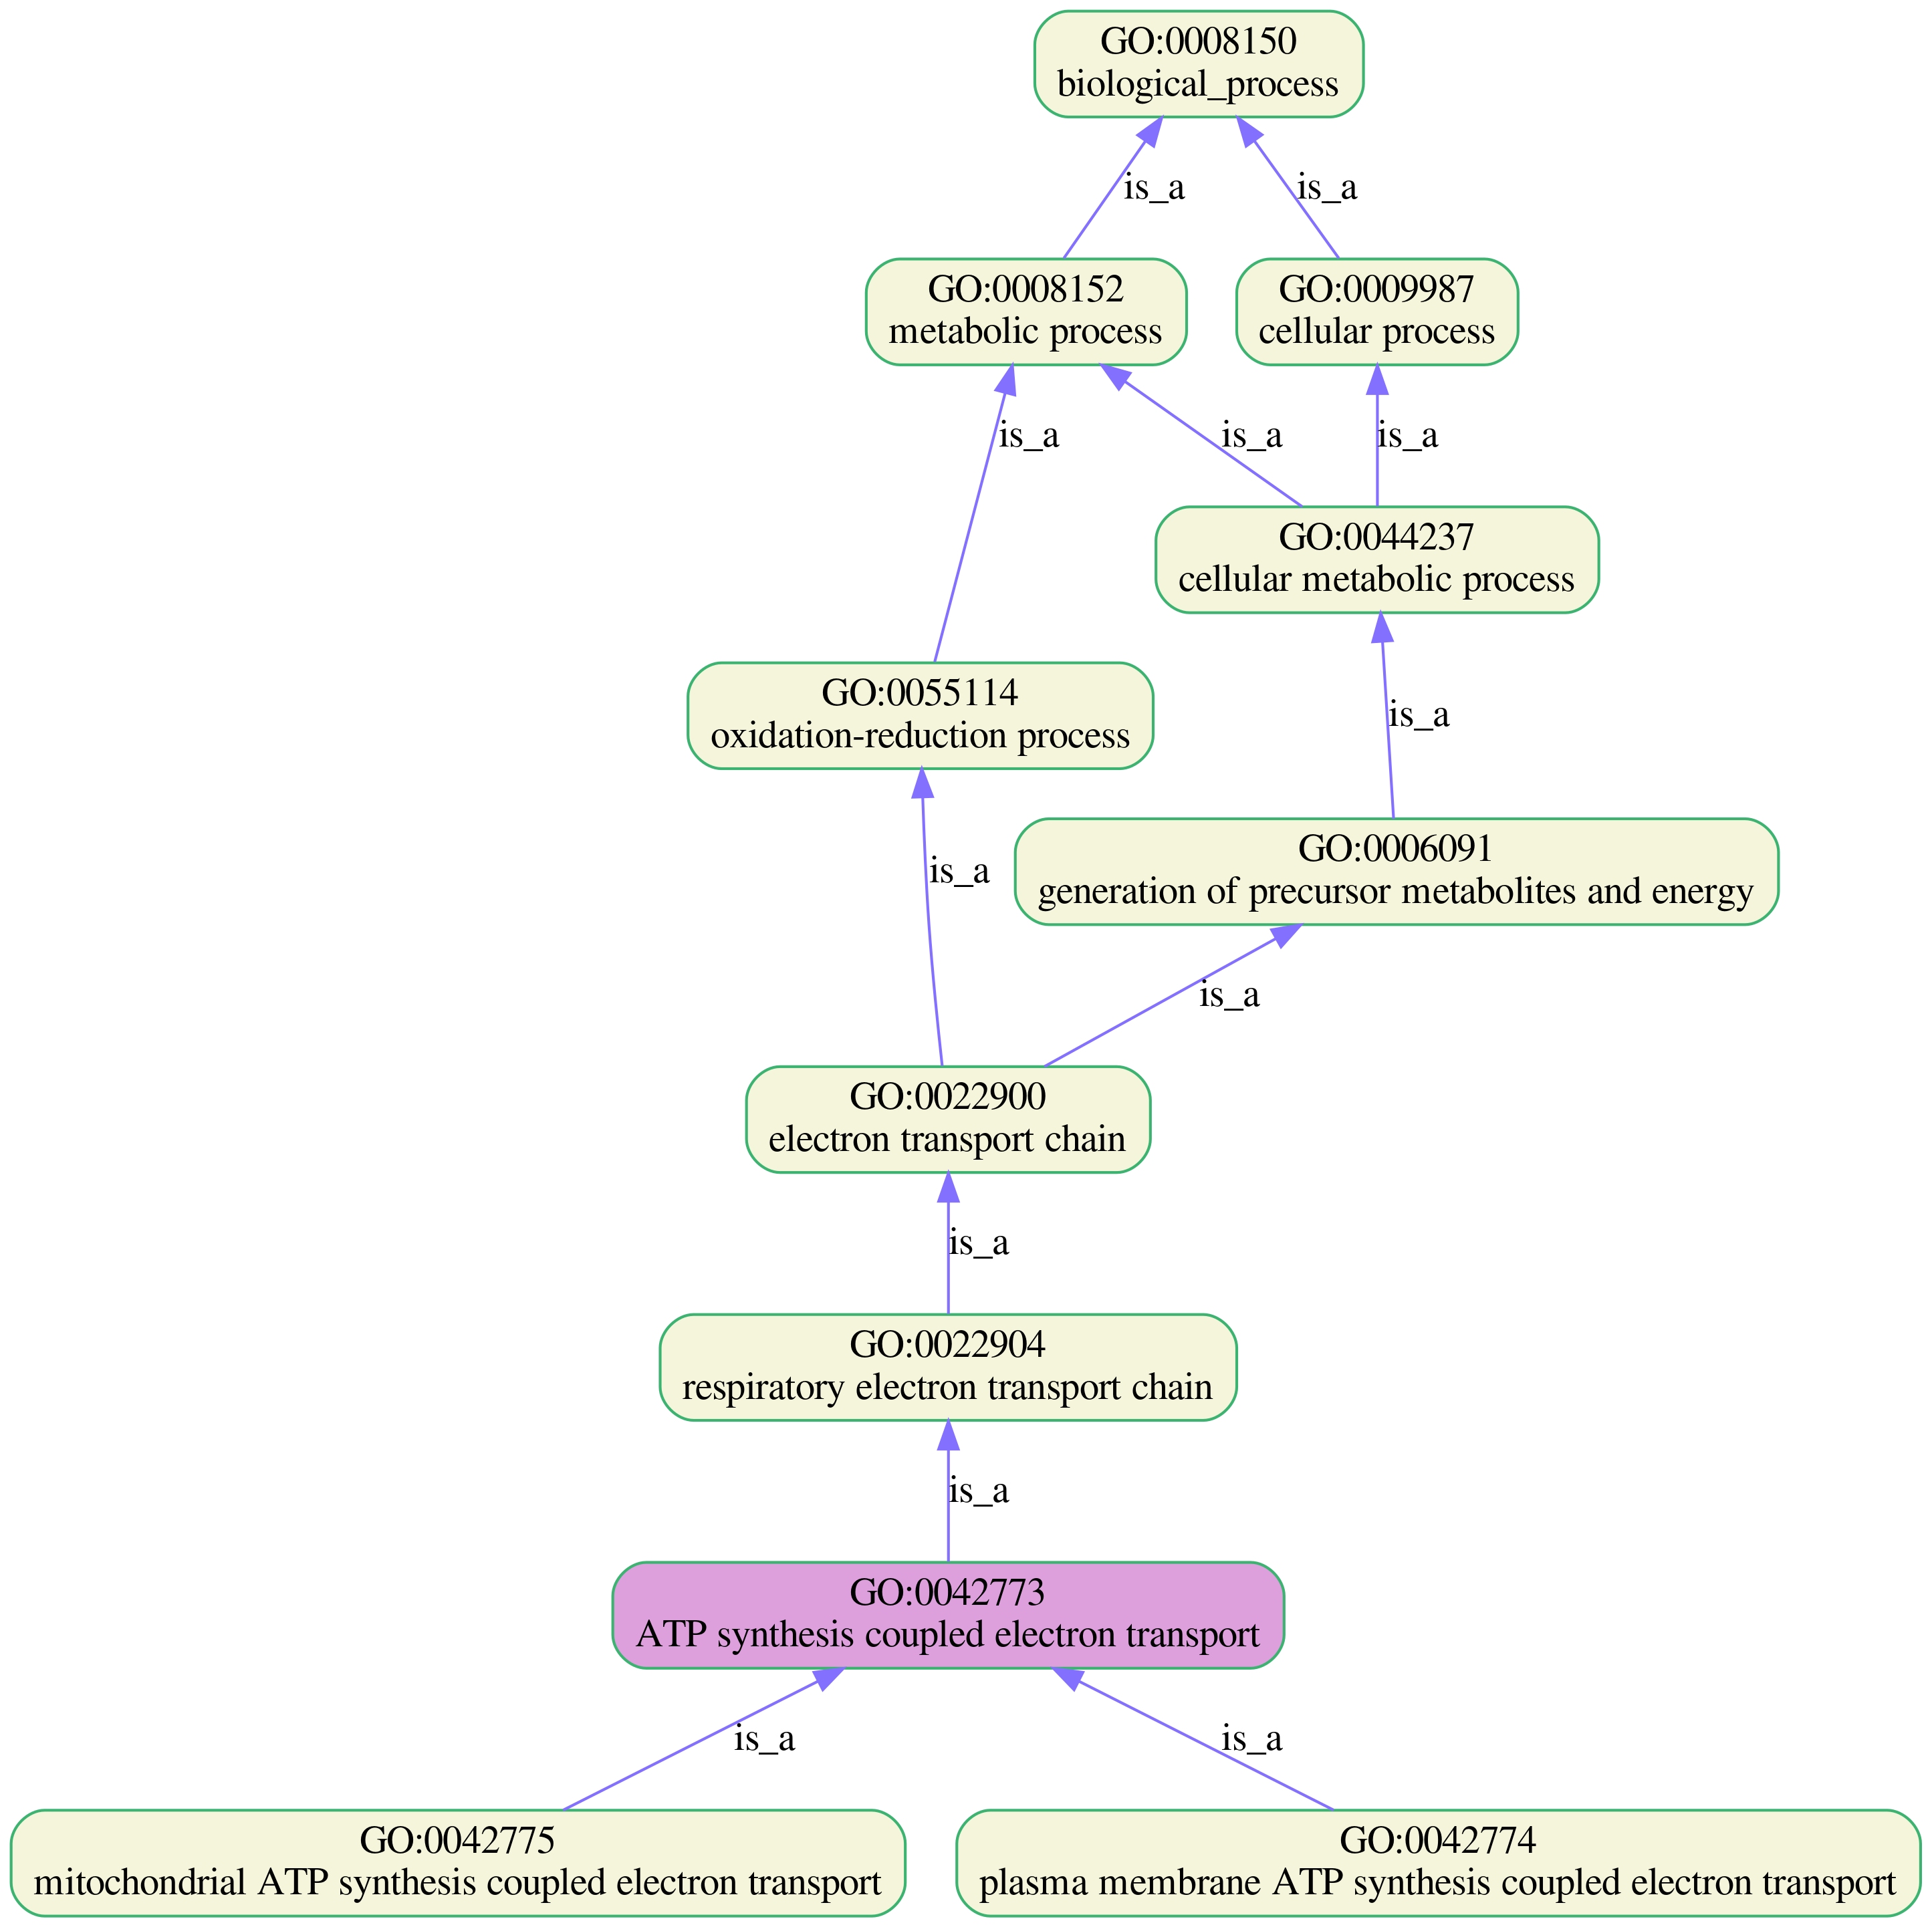
\includegraphics[scale=0.13]{GO_0042773_lineage.png}
\caption{Example of a small section of the Gene Ontology (GO), focussed GO:0042773 (in purple), showing parents and children of the term.   Generated by GOATOOLS.}
\label{fig-eg_go_graphic}
\end{center}
\end{figure}

The result of this analysis, per metagene, is a list of enriched (or depleted, however in our case no depleted terms were found) GO terms, each with an associated list of involved genes and a FDR significance level.   This list can be inspected directly for insights, but that misses the point of the GO, which is to organise the terms hierarchically by `is a' relationships.   Thus, the enriched terms were rendered graphically to show them in the context of their parent terms; an example is shown in figure \ref{fig-eg_go_graphic}


\subsection{Transfer of learned metagenes to novel a dataset}
\label{sec-transfer-to-novel}

\newcommand{\trainset}{\mathcal{T}}
\newcommand{\validset}{\mathcal{V}}

It is fundamental to our approach that \emph{metagenes} determined on the basis of one cohort of data can be used to generate \emph{metasamples} for a different cohort.  In the exposition below we refer to these as the \emph{training} and \emph{validation} cohorts respectively.

Rank $k$ matrix factorization on the training dataset $\trainset$ (e.g. TCGA) results in:
\begin{equation}
 X_\trainset \approx W_\trainset H_\trainset
\end{equation}
where $X_\trainset$ is the expression matrix of shape $(g_\trainset, n_\trainset)$, with $g_\trainset$ the number genes and $n_\trainset$ the number of patients. $W_\trainset$ is the metagene matrix of shape $(g_\trainset, k)$ and $H_t$ is the metasamples matrix of shape $(k, n_\trainset)$.

We wish to apply the factorization learned on $\trainset$ to a novel dataset $\validset$ (specifically the AOCS dataset) of shape $(g_\validset, n_\validset)$. 
Importantly, $n_\validset = 1$ reflects the application of these methods to a single patient in a clinical setting.  To apply the learned factorization we need to find $H_\validset$ as in the factorization
\begin{equation}
	X_\validset \approx W_\validset H_\validset
\end{equation}
In both the experimental and clinical situation we are given $X_\validset$ but not $W_\validset$ and require to find $H_\validset$. 
We \emph{cannot} simply perform the matrix factorization on dataset $\validset$ since $n_\validset$ may be small, or even a single patient.   
However, if patients in datasets $\trainset$ and $\validset$ are drawn from the same population (ovarian cancer patients), then $X_\trainset$ and $X_\validset$ can be expected to have similar distributions w.r.t to their columns, and thus $W_\trainset$ and $W_\validset$ can be expected to be equivalent within sampling error.  
This only makes sense if the two expression matrices $X_\trainset$ and $X_\validset$ are defined over the \emph{same set of genes}, so that $g_\trainset = g_\validset = g$, in which case $W_\trainset$ and $W_\validset$ have the same shape of $(g, k)$.   

We thus need to solve for $H_\validset$ in
\begin{equation}
	X_\validset  \approx  W_\trainset H_\validset \label{eq_Xv_WtHv}
\end{equation}

This can be solved by the method of least squares.  In the case that the original factorization was by NMF, we use non-negative least square regression (NNLS):
\begin{equation}
	H_\validset = \mbox{argmin}_{H\geq 0}{\lvert W_\trainset H - X_\validset \rvert}_2
	\label{eq_Hv_WdtXv}
\end{equation}
where ${\lvert \mathbf{\cdot} \rvert}_2$ indicates Euclidean distance or L2-norm.
The Python library function {\tt scipy.optimize.nnls} is used.

For ICA and PCA we use ordinary least square regression, formulated a above but dropping the $H\geq 0$ constraint, using {\tt scipy.linalg.lstsq}.

%An internal check on the validity of the statistical assumptions can be made my substituting  $H_\validset$ from (\ref{eq_Hv_WdtXv}) into (\ref{eq_Xv_WtHv}) and assessing the accuracy of the approximation by RMS difference.

The end result of the analysis is the $H_\validset$ matrix of shape $(k, n_\validset)$, thus delivering for each dataset in our $\validset$ a feature vector -- or metasample -- of length $k$. 

Since in this work we wish to evaluate the efficacy of the three factorization methods -- NMF, ICA and PCA -- we in fact take forward three different $H$ matrices, each having ranks as for the associated metagenes.

\subsection{Reconciling computed metasamples and metadata}
\label{sec-reconciling-metasamples-metadata}

To carry out patient level analysis -- survival analysis, heatmaps and boxplot -- as described in the following sections, it is necessary to compile tables (Pandas DataFrames) which bring together per-patient metasamples relating to each of the selected metagenes, with associated metadata -- such as cellularity and survival information.   The metagenes always derive from the TCGA dataset (because of its larger size as explained in section \ref{sec-metagene-selection}), but we wish to apply these metagenes to the expression data and associated metadata of either the TCGA or AOCS datasets.   
The mathematics of transferring metagenes across datasets has been described above.  Care is required to ensure that expression matrices are aligned correctly with metagenes with respect to their genes (rows), and with the metadata with respect to patient identifiers in the columns.
Note that the same transferring approach is taken when metasamples are required for TCGA, even though we could in that case obtain the $H$ matrix directly from the factorization.


\subsection{Survival analysis}
\label{sec-survival-analysis}

Survival analysis was performed to investigate whether the metasamples derived from the selected metagenes correlate with patient survival.  Overall  survival (OS) data is available for both the TCGA and AOCS datsets.  Additionally, progression free survival (PFS) data is available for AOCS.   As described above,  metagenes were obtained by factorization on the TCGA dataset only.  Application to TCGA (for OS) thus represents an in-sample test, while application to AOCS (for OS and PFS) is a more exacting out-of-sample test. There are thus three analyses to consider: 1) TCGA$\rightarrow$TCGA (OS), 2) TCGA$\rightarrow$AOCS (OS) and 3) TCGA$\rightarrow$AOCS (PFS). \emph{TODO: describe these three versions of analysis in words}.

Analysis was performed using the Python {\tt Lifelines} package \cite{Davidson-Pilon2020}.  %Metasamples ($H$ matrices) were calculated from the metagenes and expression matrix as explained in section \ref{sec-transfer-to-novel} below.  
Metasample values were binariased to 0, 1 by thresholding at the median value.   Kaplan-Meier plots were made in respect of derived metasample for each of the three analyses -- making $11 \times 3$ plots each with two survival curves with 95\% confidence intervals.  A hazard ratio (HR)
was calculated for each plot by fitting Cox's proportional hazards model with p-value relating to the hypothesis that HR is significantly different to 1.0.


\subsection{Investigating correlation between metasamples and genomic features}

For the AOCS dataset (only) pre-determined per-patient high-level genomic features were available as follows:
\begin{description}
\item[WGD]: Whole genome doubling -- a marker of genome instability.  This is a binary feature.
\item[Cellularity]: proportion of cells belonging to the tumour (as opposed to surrounding normal tissue).
\item[HR Detect]: A predictor of homologous repair deficiency based on established mutational features \cite{Ewing2020}.
\item[Mutational Load]: A measure of the total number of mutations present in the tumour genome.
\item[CNV Load]: Copy-number variation, i.e. deviation from the normal diploid cell compliment.
\item[SV Load]: Structural variation, a measure of the degree of chromosomal rearrangements such as translocations and inversions.
\end{description}

Scatter plots were generated between each metasample and each genomic features -- a grid of $11 \times 6 = 66$ plots in all.  These were based on the reconciled metasamples and metadata as described in section \ref{sec-reconciling-metasamples-metadata}.  Pearson's correlation coefficients ($r$) and associated p-values (i.e. the probability that $r$ does not differ from zero) were calculated.   However, since WGD is a binary feature, the more appropriate Point-Biserial correlation was used in that case.  A p-value significance threshold of 0.01 was chosen, although with 66 hypotheses being tested, this does risk false discovery.

As an alternative visualisation of the relationship between metasamples and genomic features, and to see the relationship between metasamples themselves, a clustered heatmaps was generated using the \href{https://seaborn.pydata.org/generated/seaborn.clustermap.html}{Seaborn {\tt clustermap()}} function based on the same underlying data as above.  


\subsection{Codebase and plotting conventions}

The described methodology was implemented in Python.
%except for the KEGG gene enrichment analysis which was implemented in R.
All code is available in a github repository: \url{https://github.com/ipoole/HgsocTromics}.  Good software engineering practice has been followed, with an object-oriented design, frequent commits and unit testing.  Unit tests are based on tiny expression matrices, just 100 genes by 10 patients, thus the whole test suite of over 60 tests executes in around 40 seconds and can be run frequently.  These tests are particularly valuable when re-factoring code.  The total codebase is approximately 2,900 lines of Python.  

All plots are generated in vector graphics pdf format to ensure smooth scaling to any resolution.  A consistent colour scheme of \textcolor{blue}{blue}, \textcolor{orange}{orange} and \textcolor{olive}{green} was used for plots relating to NMF, ICA and PCA respectively.  Metagenes are consistently referred to by, for example, ``NMF-2-of-3" -- meaning the 2nd component of the rank $k=3$ NMF factorization.


%%%%%%%%%%% RESULTS %%%%%%%%%%%%%
\clearpage

\section{Results}


% \subsection{Investigation of optimal parameters}
\subsection{Consideration of sampling error is crucial to finding robust metagene signals}

From figure \ref{fig-AOCS-ica-fixed-vs-bootstrap} it can be seen that with sampling error excluded, clusters appear reasonably coherent, but when sampling error is modelled by bootstrap sampling then  the factorizations become much less stable.  This demonstrates that \emph{sampling} error is far greater than errors due to algorithm initialisation when the dataset is small (N=80), making metagene extraction unreliable.   Figure  \ref{fig-TCGA-ica-fixed-vs-bootstrap} makes the same comparison for the lager N=374 TCGA dataset, in which it can be seen that the impact of sampling error is not so severe.  For brevity only results for ICA are shown here; similar result for PCA and NMF can be found in the appendix, figures

For this reason it is appropriate to perform all metagene extraction on the larger TCGA dataset, in the expectation that the obtained metagenes will be more robust and likely to better generalise to other datasets.

\def\S{0.45}
\begin{figure}[ht]
\begin{center}
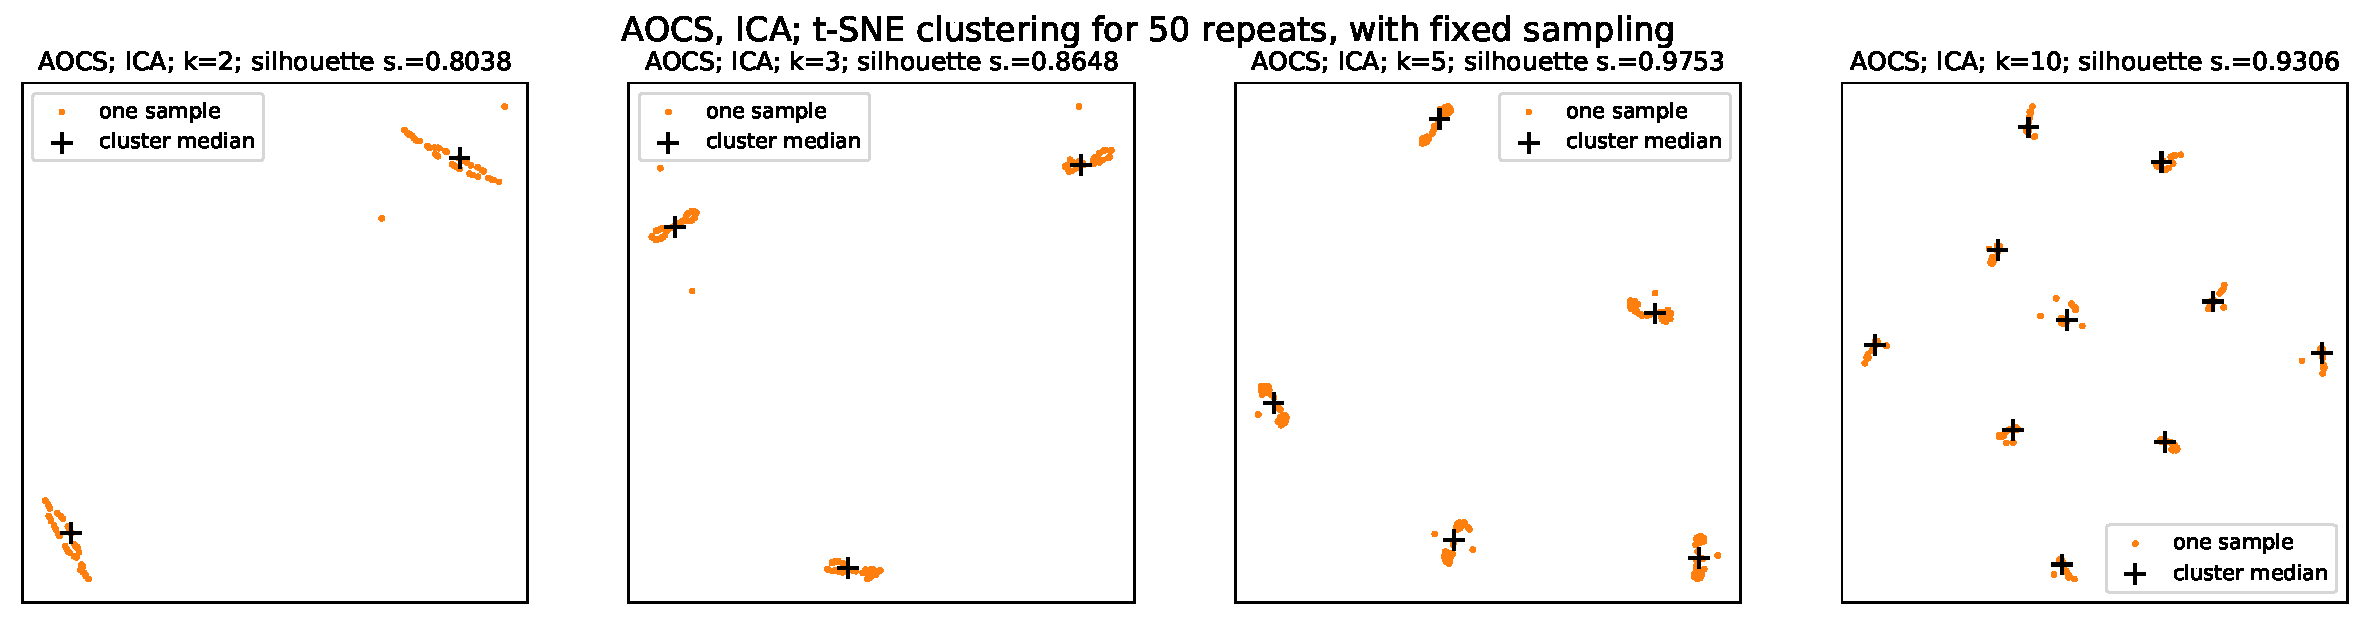
\includegraphics[scale=\S]{\plotspath{AOCS_Protein/FactorClustering/multiple_single_factors_scatter_AOCS_ICA_2_3_5_10_fixed.pdf}} \\
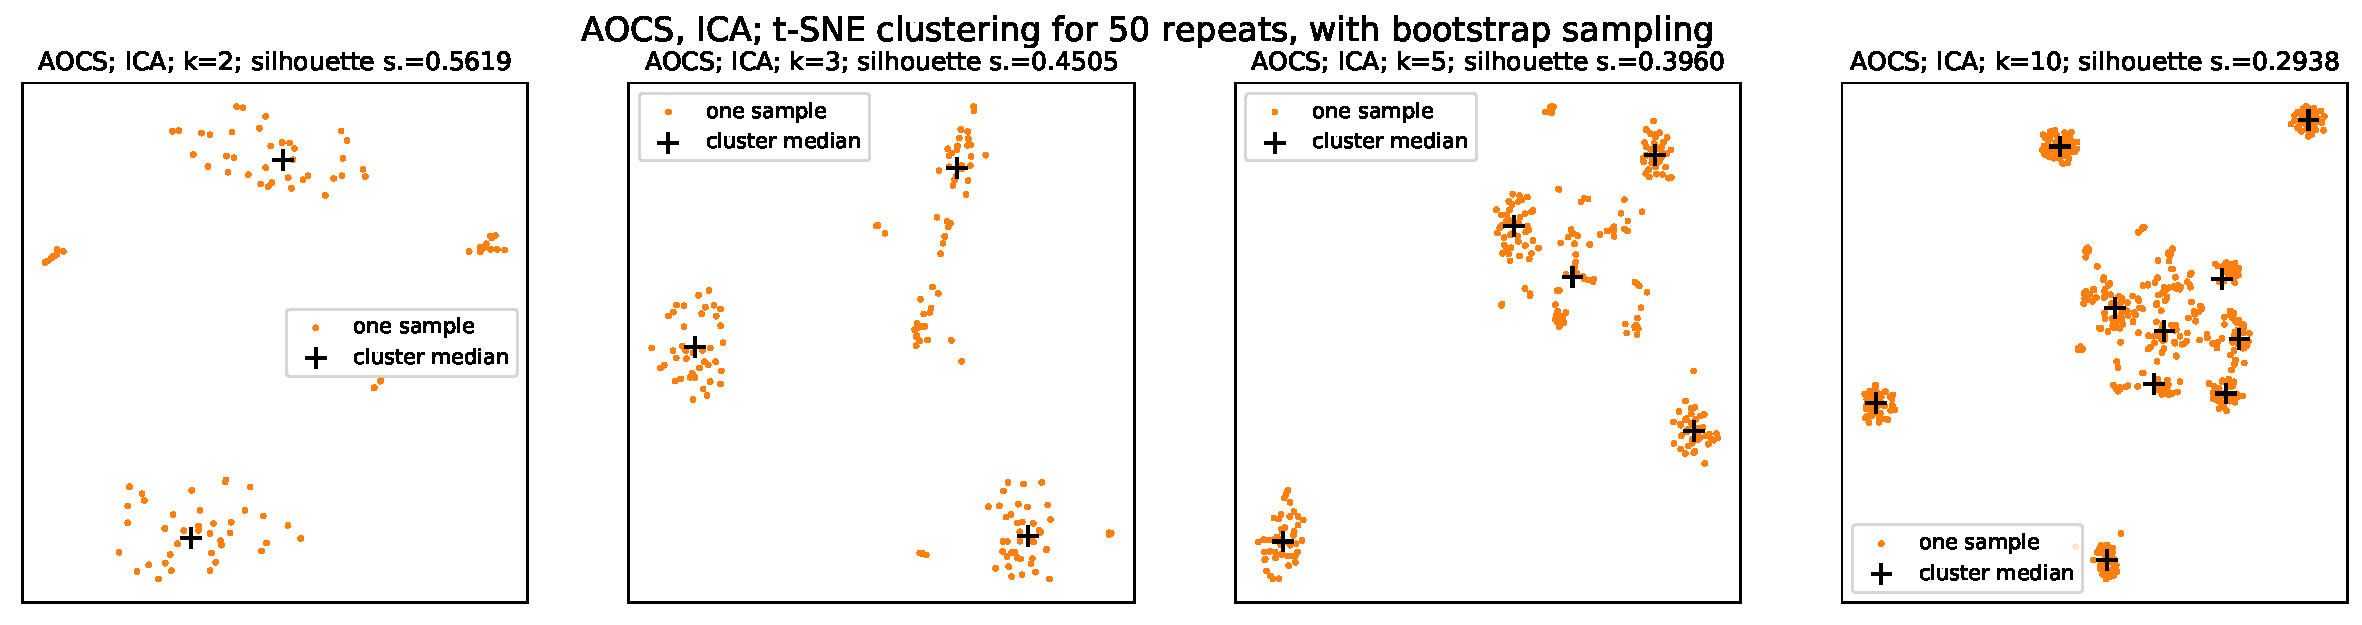
\includegraphics[scale=\S]{\plotspath{AOCS_Protein/FactorClustering/multiple_single_factors_scatter_AOCS_ICA_2_3_5_10_bootstrap.pdf}}\\
\caption{Clustering of metagenes from ICA facorizations on the N=80 AOCS dataset, comparing \emph{fixed} sampling (top row) with \emph{bootstrap} sampling (bottom row) for a selection of factorization ranks.  }
\label{fig-AOCS-ica-fixed-vs-bootstrap}
\label{fig-first-cluster-result}
\end{center}
\end{figure}

\begin{figure}[ht]
\begin{center}
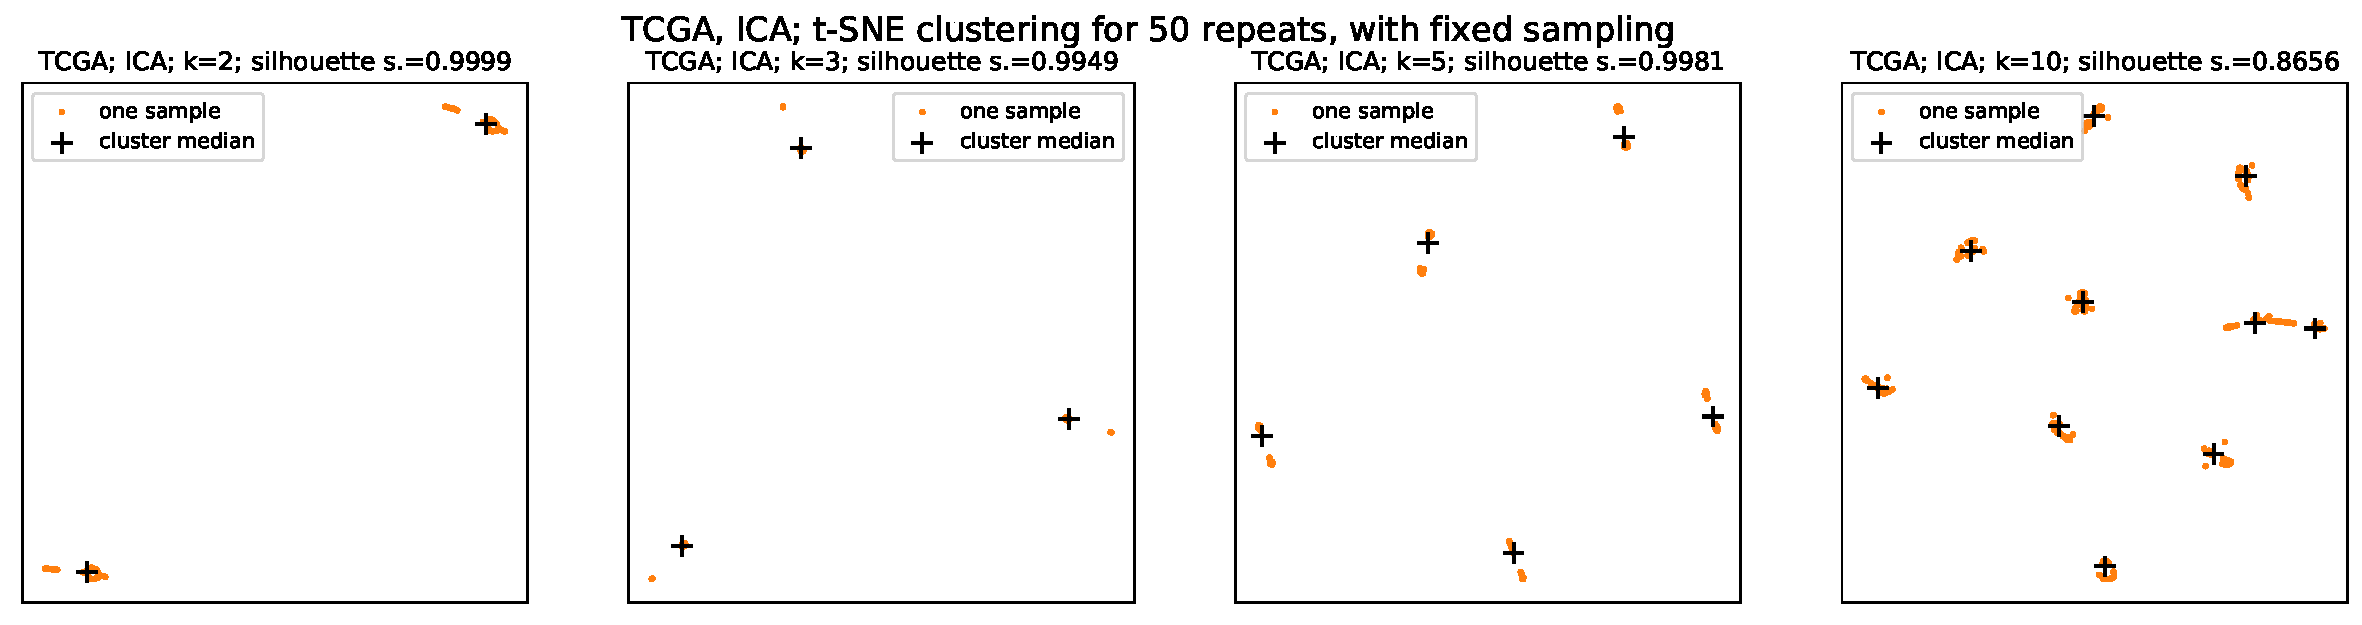
\includegraphics[scale=\S]{\plotspath{TCGA_OV_VST/FactorClustering/multiple_single_factors_scatter_TCGA_ICA_2_3_5_10_fixed.pdf}} 
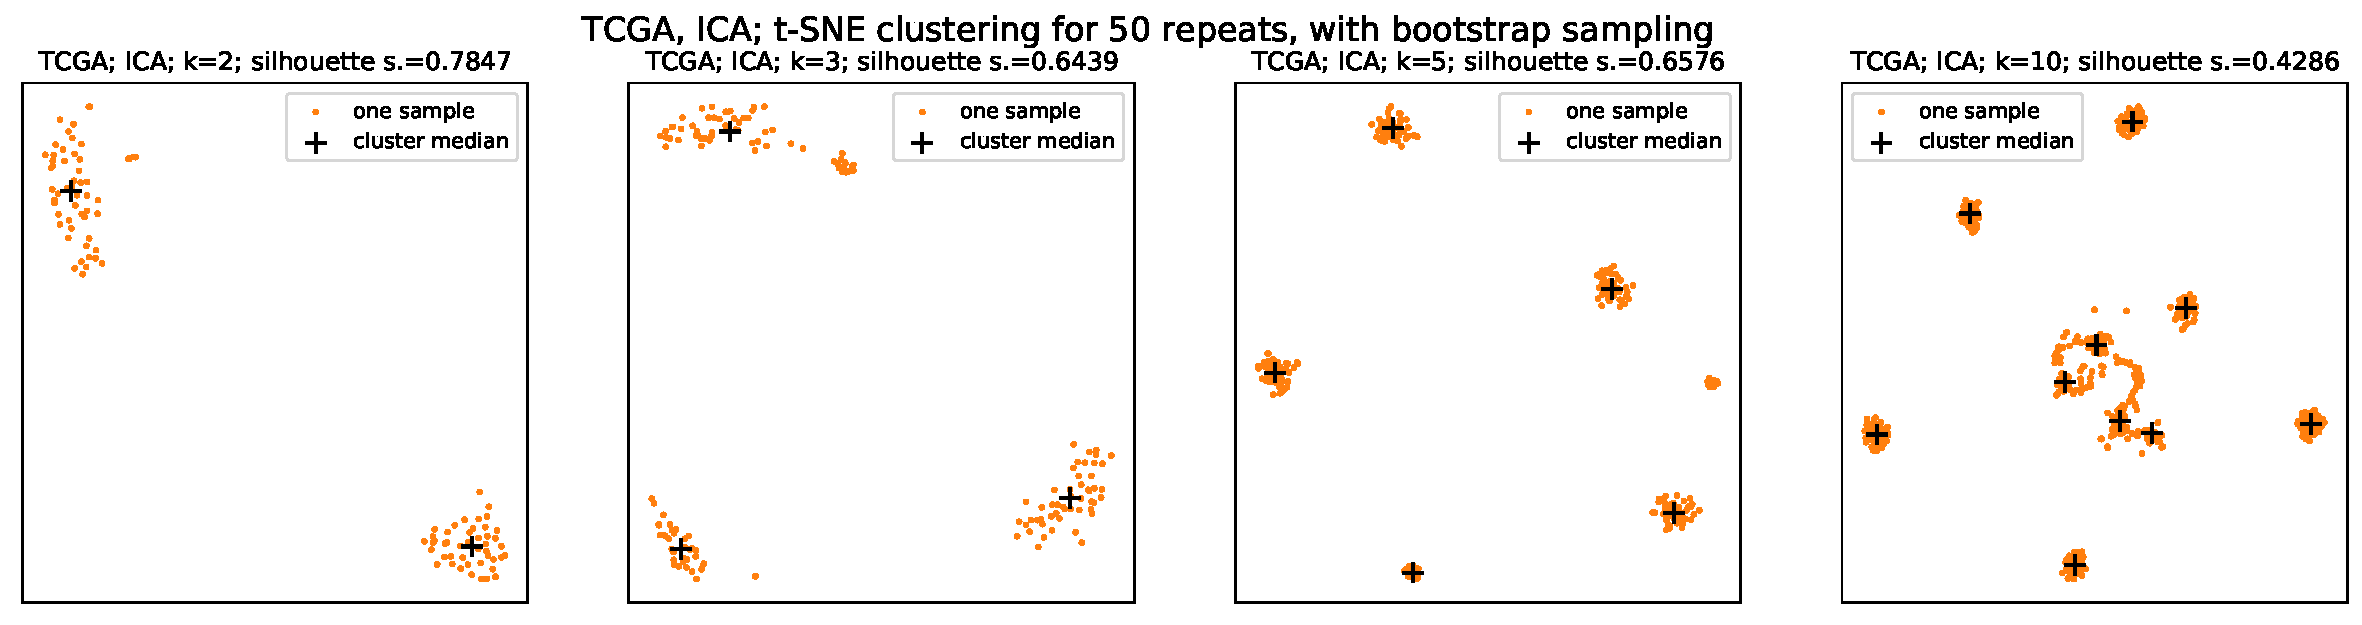
\includegraphics[scale=\S]{\plotspath{TCGA_OV_VST/FactorClustering/multiple_single_factors_scatter_TCGA_ICA_2_3_5_10_bootstrap.pdf}}
\caption{Clustering of metagenes from ICA facorizations on the N=374 TCGA dataset, again comparing fixed and bootstrap sampling.}
\label{fig-TCGA-ica-fixed-vs-bootstrap}
\end{center}
\end{figure}


In choosing the factorization rank for each method, both the t-SNE plots and silhouette scrore graphs in  figure \ref{fig-TCGA-all-bootstrap} were carefully considered.  
Firstly, $k>2$ is desirable to have sufficient information to work with.  NMF cluster coherence seems to deteriorate after $k=3$.   Looking at the graph of silhouette scores (figure \ref{fig-TCGA-all-bootstrap}, bottom), ICA appears to have a sweet spot at $k=5$.  For PCA, $k = 3$ or $4$ both seem reasonable.
The following choices were made:
$K_{\mbox{\tiny NMF}}  =  3,
K_{\mbox{\tiny ICA}}  =  5,
K_{\mbox{\tiny PCA}}  =  3$.  These choices predicate all the results which follow.

There is a curious artefact visible in the NMF factorization clusterings of figure \ref{fig-TCGA-all-bootstrap}, top row.  For $k=2, 3$ and $5$ several of the clusters show a bi-modal character.  This is not observed in the fixed sampling case (not shown).  The artefact is difficult to explain.  It cannot be the $180^\circ$ rotation issue discussed earlier, since this does not apply to the all +ve components. \emph{TODO: hypothesis?}

\begin{figure}[ht]
\begin{center}
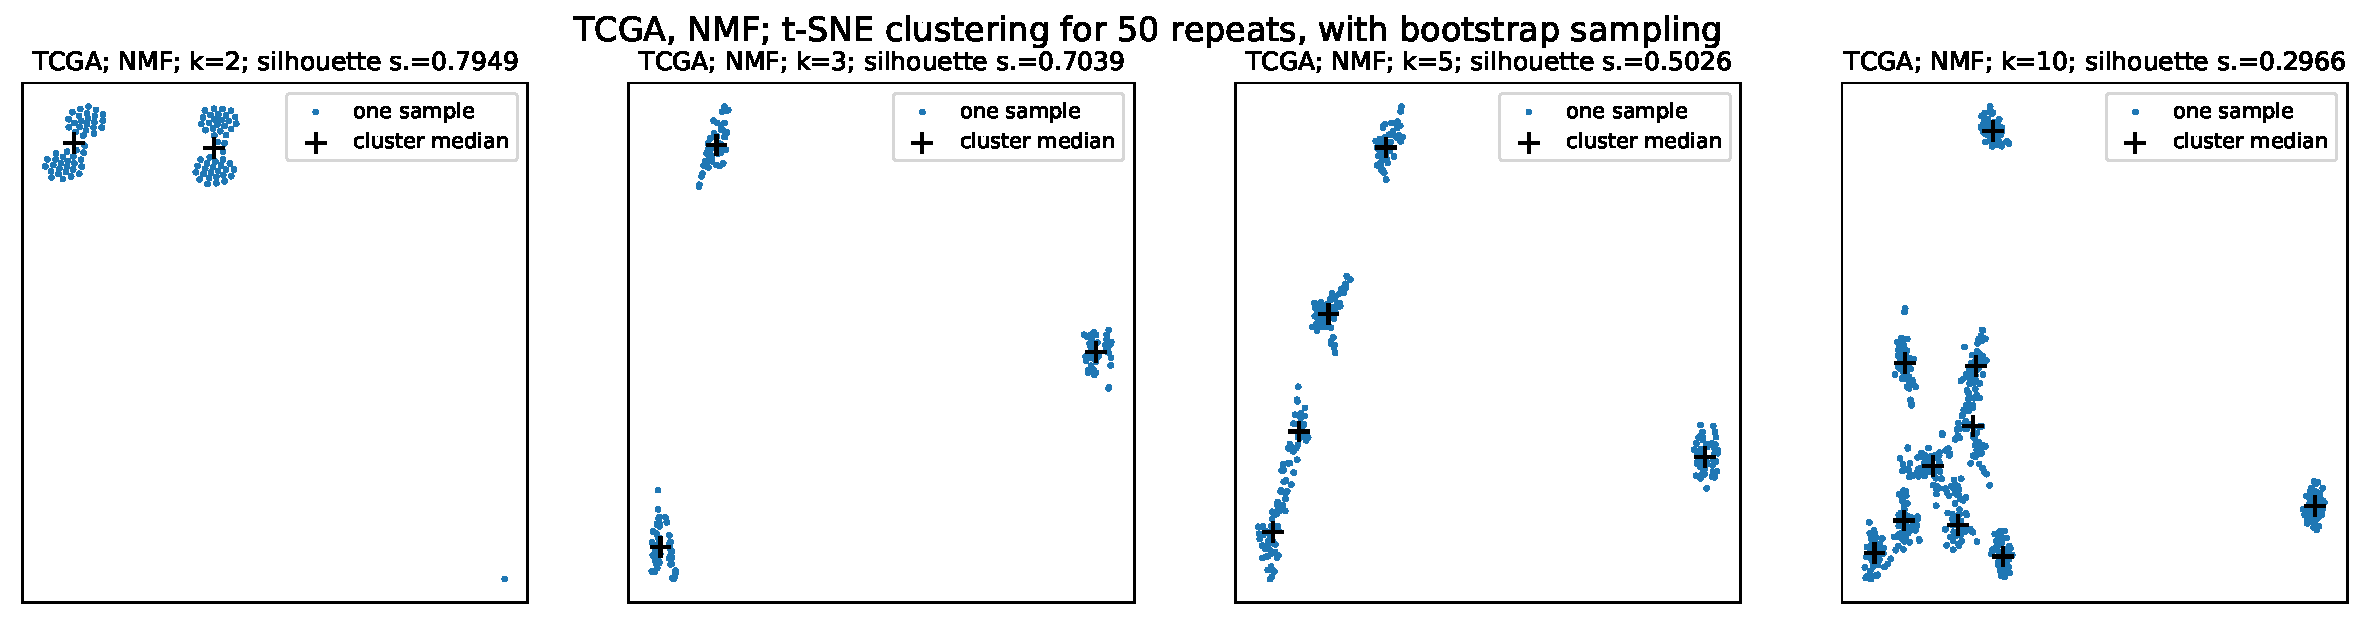
\includegraphics[scale=\S]{\plotspath{TCGA_OV_VST/FactorClustering/multiple_single_factors_scatter_TCGA_NMF_2_3_5_10_bootstrap.pdf}} \\
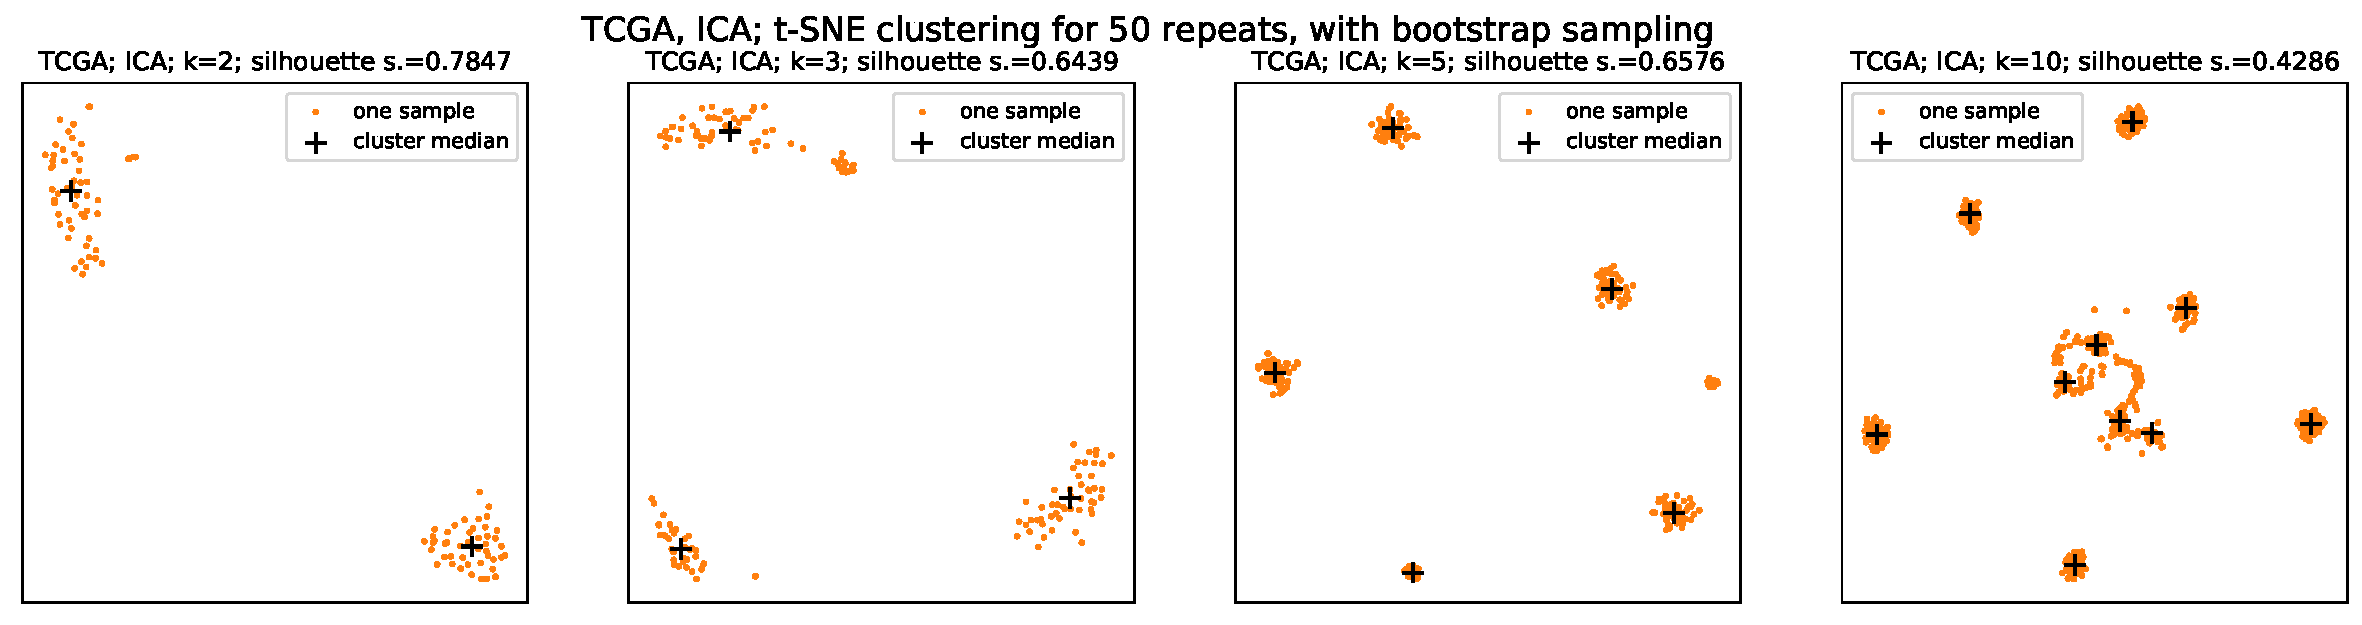
\includegraphics[scale=\S]{\plotspath{TCGA_OV_VST/FactorClustering/multiple_single_factors_scatter_TCGA_ICA_2_3_5_10_bootstrap.pdf}} \\
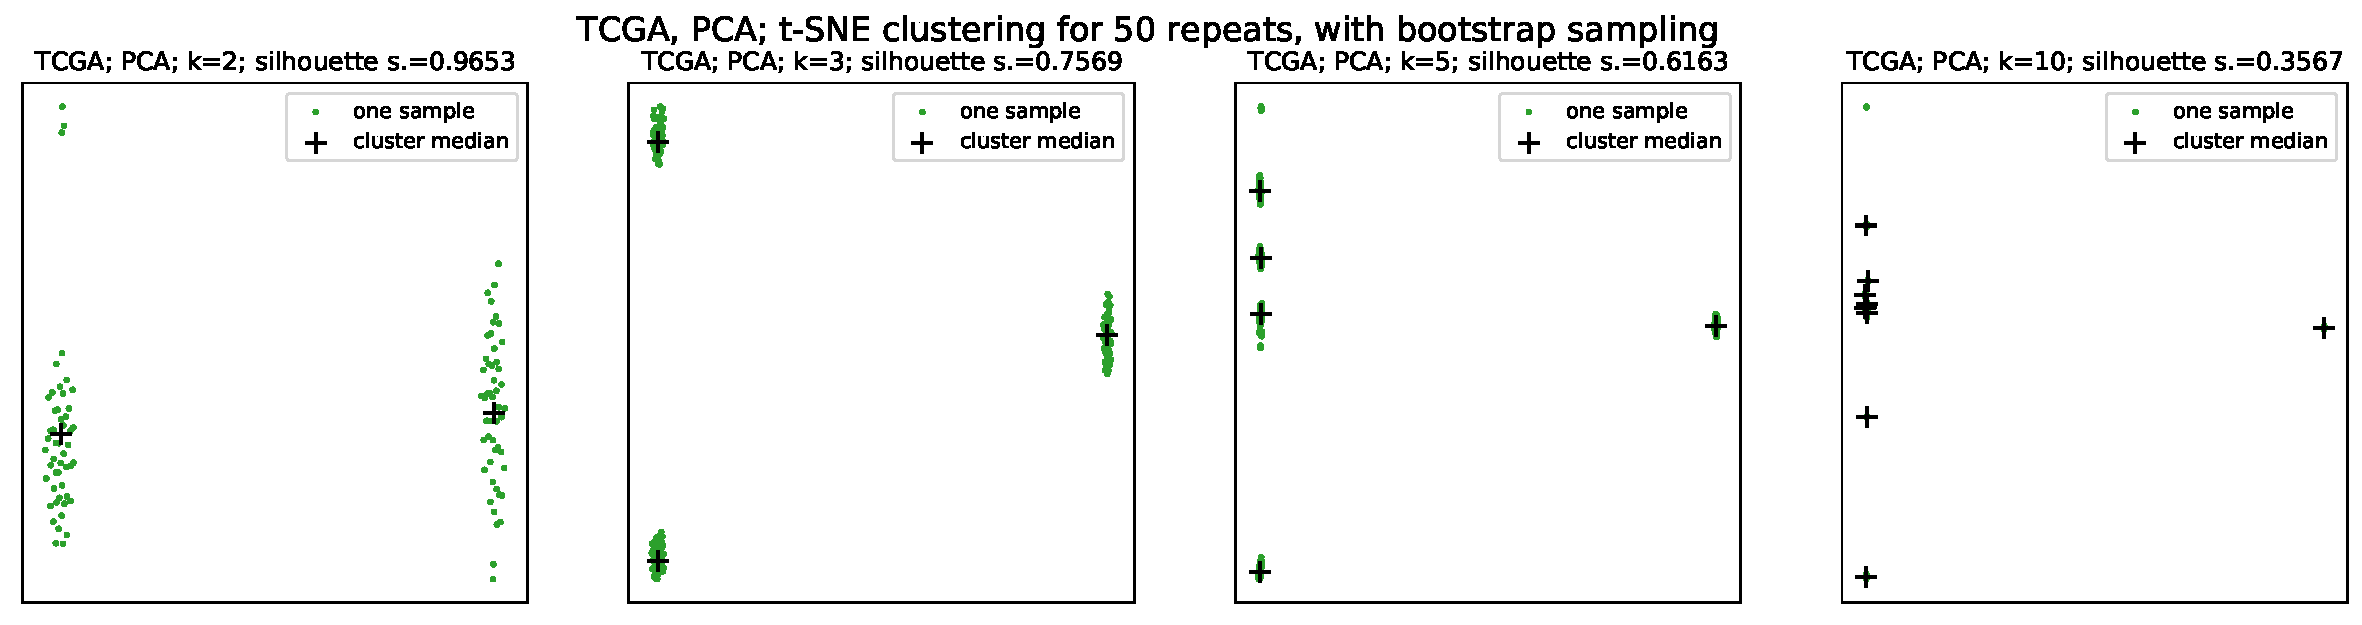
\includegraphics[scale=\S]{\plotspath{TCGA_OV_VST/FactorClustering/multiple_single_factors_scatter_TCGA_PCA_2_3_5_10_bootstrap.pdf}} \\
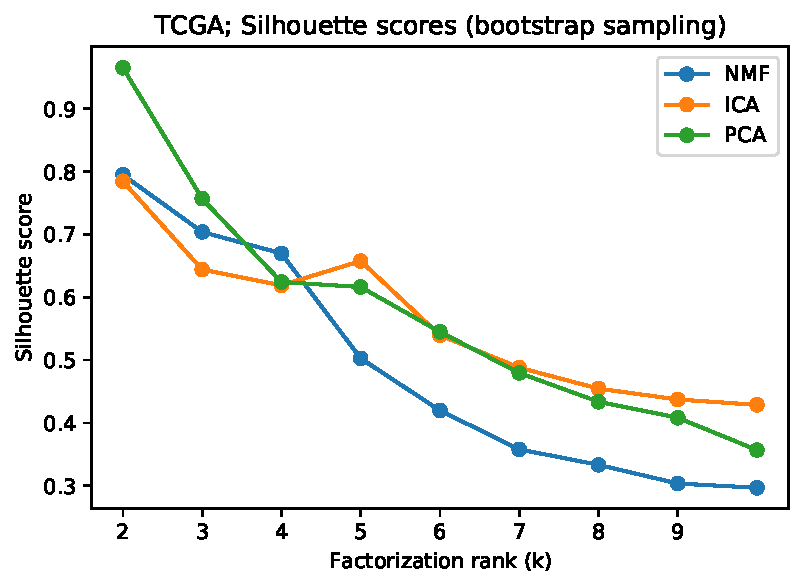
\includegraphics[scale=0.55]{\plotspath{/TCGA_OV_VST/FactorClustering/silhouette_plots_TCGA_2_3_4_5_6_7_8_9_10_bootstrap.pdf}} 
\caption{Metagene clustering for all three methods applied to the N=374 TCGA dataset with bootstrap sampling, over a range of factorization ranks.  The silhouette scores are also plotted (bottom).  It is on the basis of this figure that the factorization ranks for each method were selected.}
\label{fig-TCGA-all-bootstrap}
\label{fig-last-cluster-result}
\end{center}
\end{figure}

\subsection{Gene sets identified by metagenes of different methods intersect in some cases}

The Jaccard heatmap of figure \ref{fig-component-jaccard-similarities} shows that some pairs of metagenes identify overlapping sets of genes, in particular the pairs (ICA-1-of-5, PCA-2-of-3: J=0.61) and (ICA-5-of-5, PCA-3-of-3: J=0.49).  As expected however, there is very little similarity between components \emph{within} a factorization method.

\begin{figure}[ht]
\begin{center}
\includegraphics[scale=0.5]{\plotspath{TCGA_OV_VST/GeneEnrichment/component_jaccard_heatmap.pdf}}
\end{center}
\caption{Heatmap of Jaccard similarities between the candidate genes identified by the 11 components.}
\label{fig-component-jaccard-similarities}
\end{figure}

\clearpage

\subsection{Metagenes highlight genes which are enriched for particular biological processes}

Gene enrichment analysis against the GO results in, for each of the 11 metagenes, a table of GO terms with a list of the candidate genes which have an annotated association to that term; this table can be found in the appendix, table \ref{tab-go-enrichment-results}.
To take full advantage of the hierarchical nature of the GO, results are presented as lineage maps in figures \ref{fig-NMF-go-lineage} to \ref{fig-PCA-1-3-go-lineage}.  
The contributing candidate genes for all significantly enriched terms are shown beneath each figure.  
High-level terms at depth less than 3 were removed, since these are generic (e.g. "regulation of biological process") and so uninteresting.   
One component -- ICA-4-of-5 -- was problematic in that 49 GO terms (with depth $\geq 3$) were identified as significant.  
For this component it was necessary to limit the graphic to the 12 terms having the largest number of associated candidate genes.   

The four components NMF-3-of-3, ICA-1-of-5, ICA-2-of-5 and PCA-2-of-3 yielded no significant enriched terms (for FDR $\leq$ 0.01).

\begin{figure}[ht]
\begin{center}
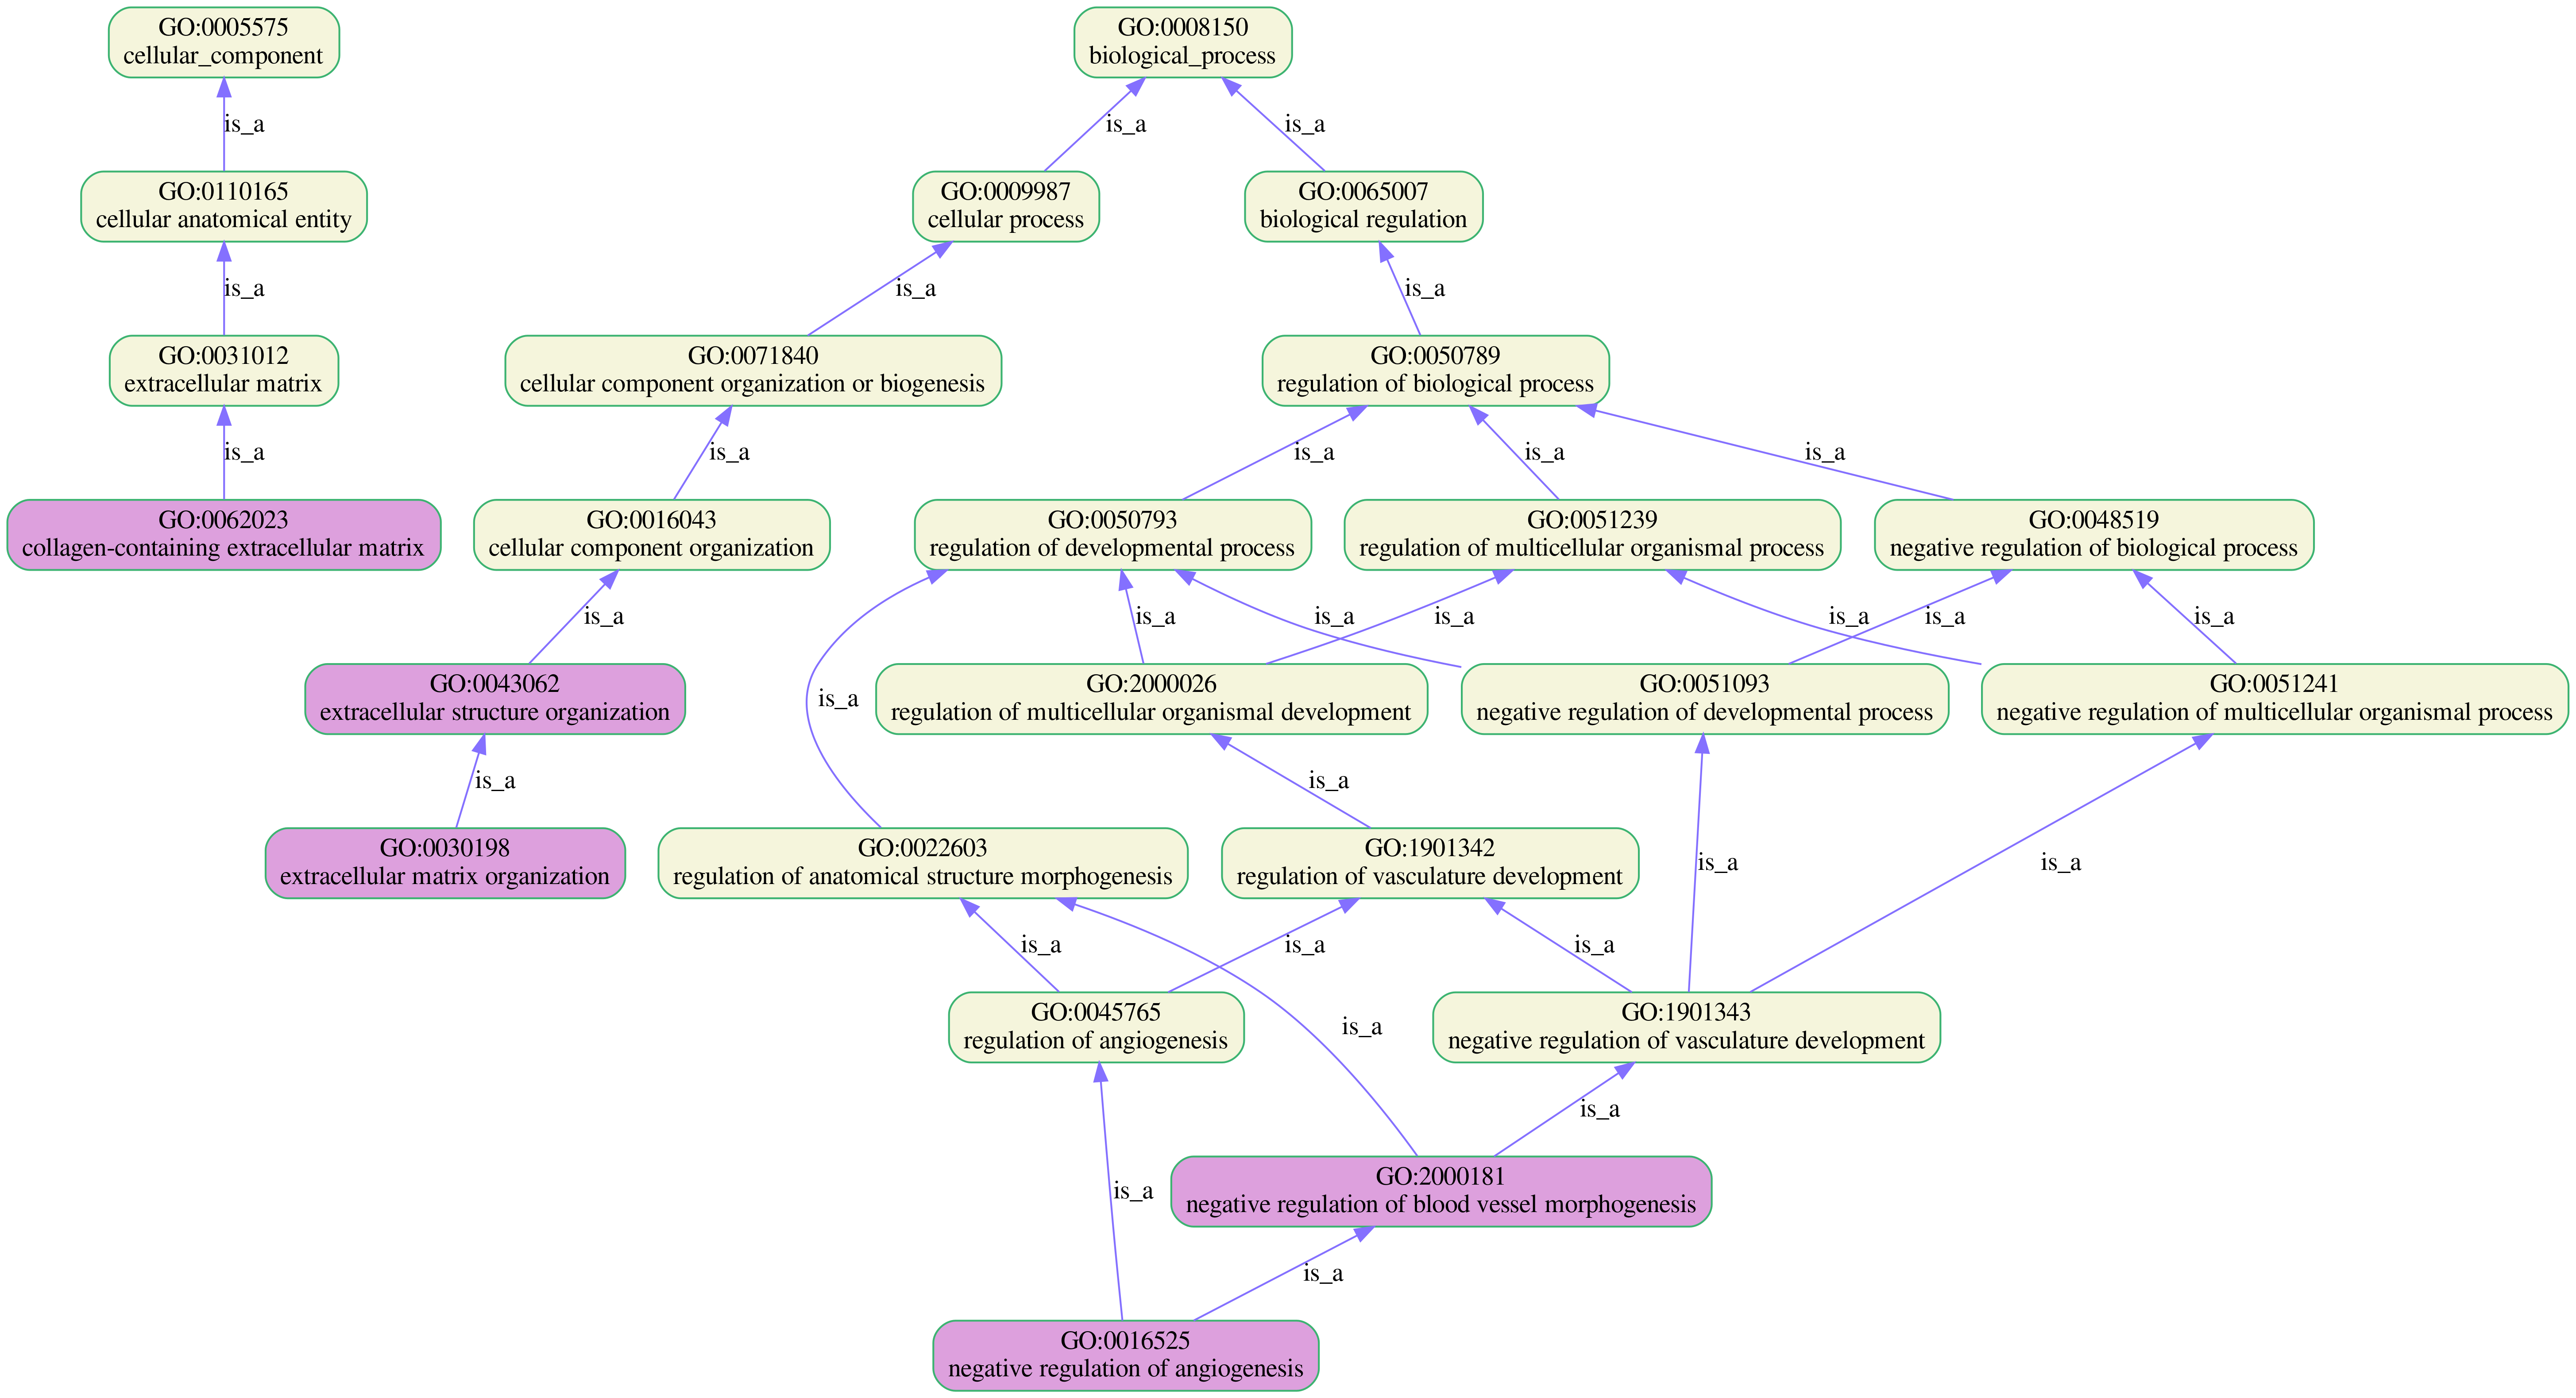
\includegraphics[scale=0.14]{\plotspath{TCGA_OV_VST/GeneEnrichment/go_lineage_1_of_NMF_3.png}} \\
\begin{spacing}{0.6}
{\small Genes: \tiny \input{/home/ipoole/Documents/gitrepos/HgsocTromics/Plots/TCGA_OV_VST/GeneEnrichment/go_gene_set_1_of_NMF_3.txt}}
\end{spacing}
\vspace{0.5cm}
{\small Component NMF-1-of-3} \\
\vspace{1cm}
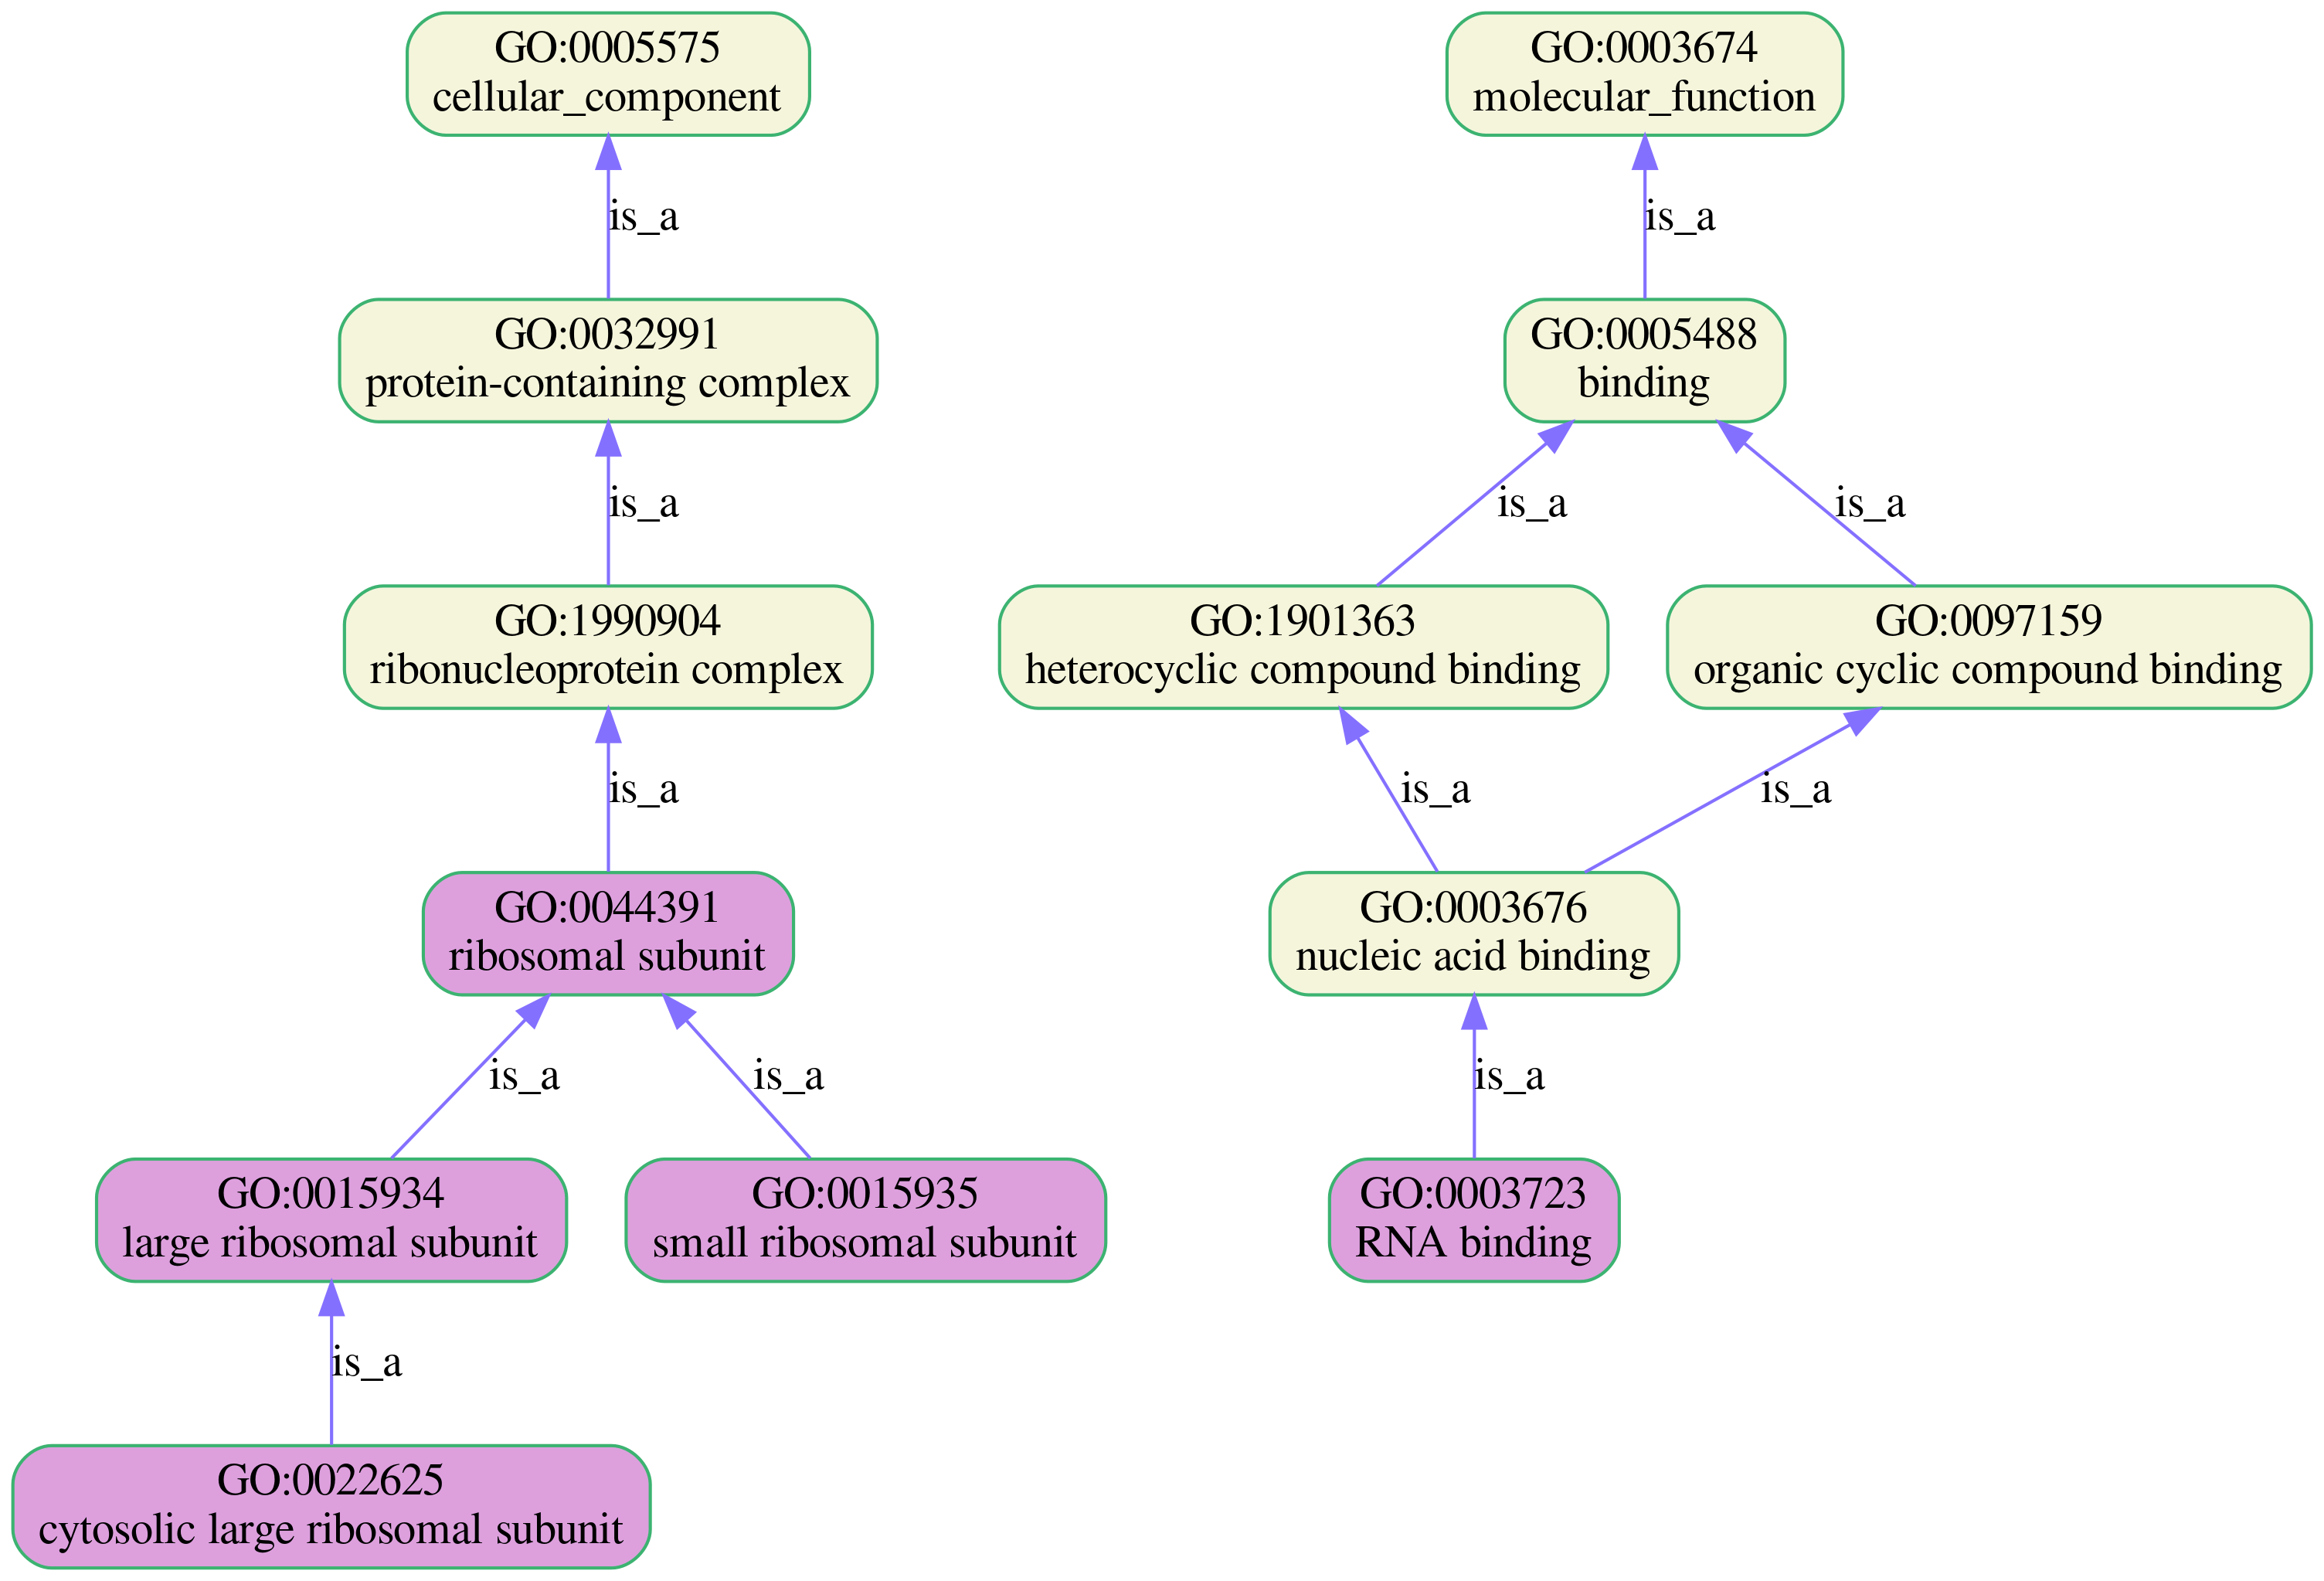
\includegraphics[scale=0.14]{\plotspath{TCGA_OV_VST/GeneEnrichment/go_lineage_2_of_NMF_3.png}} \\
\begin{spacing}{0.6}
{\small Genes: \tiny \input{/home/ipoole/Documents/gitrepos/HgsocTromics/Plots/TCGA_OV_VST/GeneEnrichment/go_gene_set_2_of_NMF_3.txt}}
\end{spacing}
\vspace{0.5cm}
{\small Component NMF 2-of-3} \\
\caption{Lineage maps of enriched Gene Ongology (GO) terms for components NMF-1-of-3 and NMF-2-of-3.  In these diagrams, enriched terms are coloured purple, while there ancestors in the ontology are yellow.  (NMF-3-of-3 produced no significant enrichment results)}
\label{fig-NMF-go-lineage}
\end{center}
\end{figure}


\begin{figure}[ht]
\begin{center}
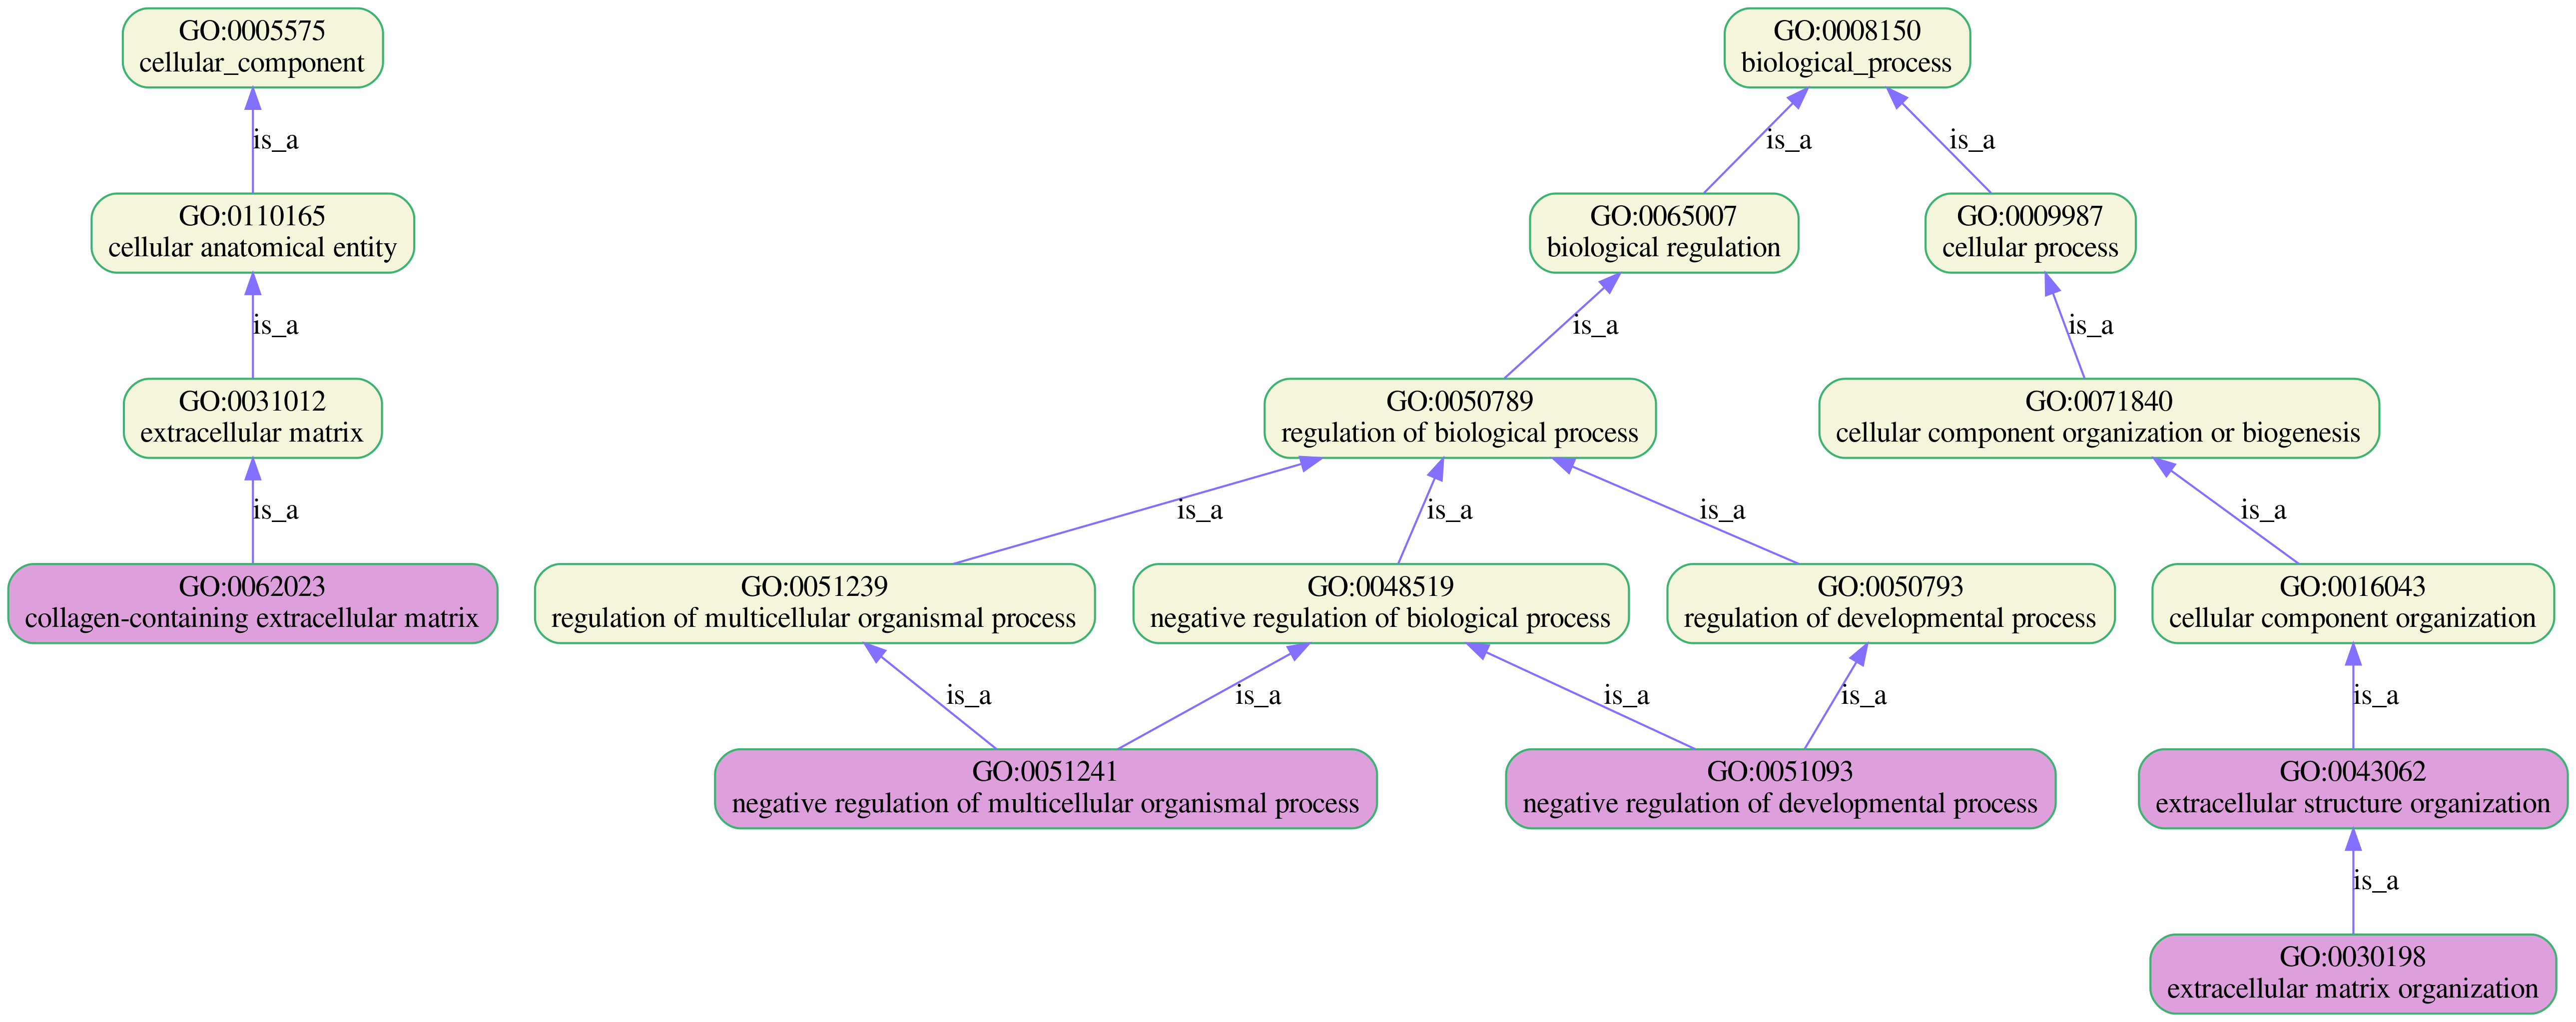
\includegraphics[scale=0.1]{\plotspath{TCGA_OV_VST/GeneEnrichment/go_lineage_3_of_ICA_5.png}} \\
\begin{spacing}{0.6}
{\small Genes: \tiny \input{/home/ipoole/Documents/gitrepos/HgsocTromics/Plots/TCGA_OV_VST/GeneEnrichment/go_gene_set_3_of_ICA_5.txt}}
\end{spacing}
\vspace{0.5cm}
{\small Component ICA-3-of-5} \\
\vspace{1cm}
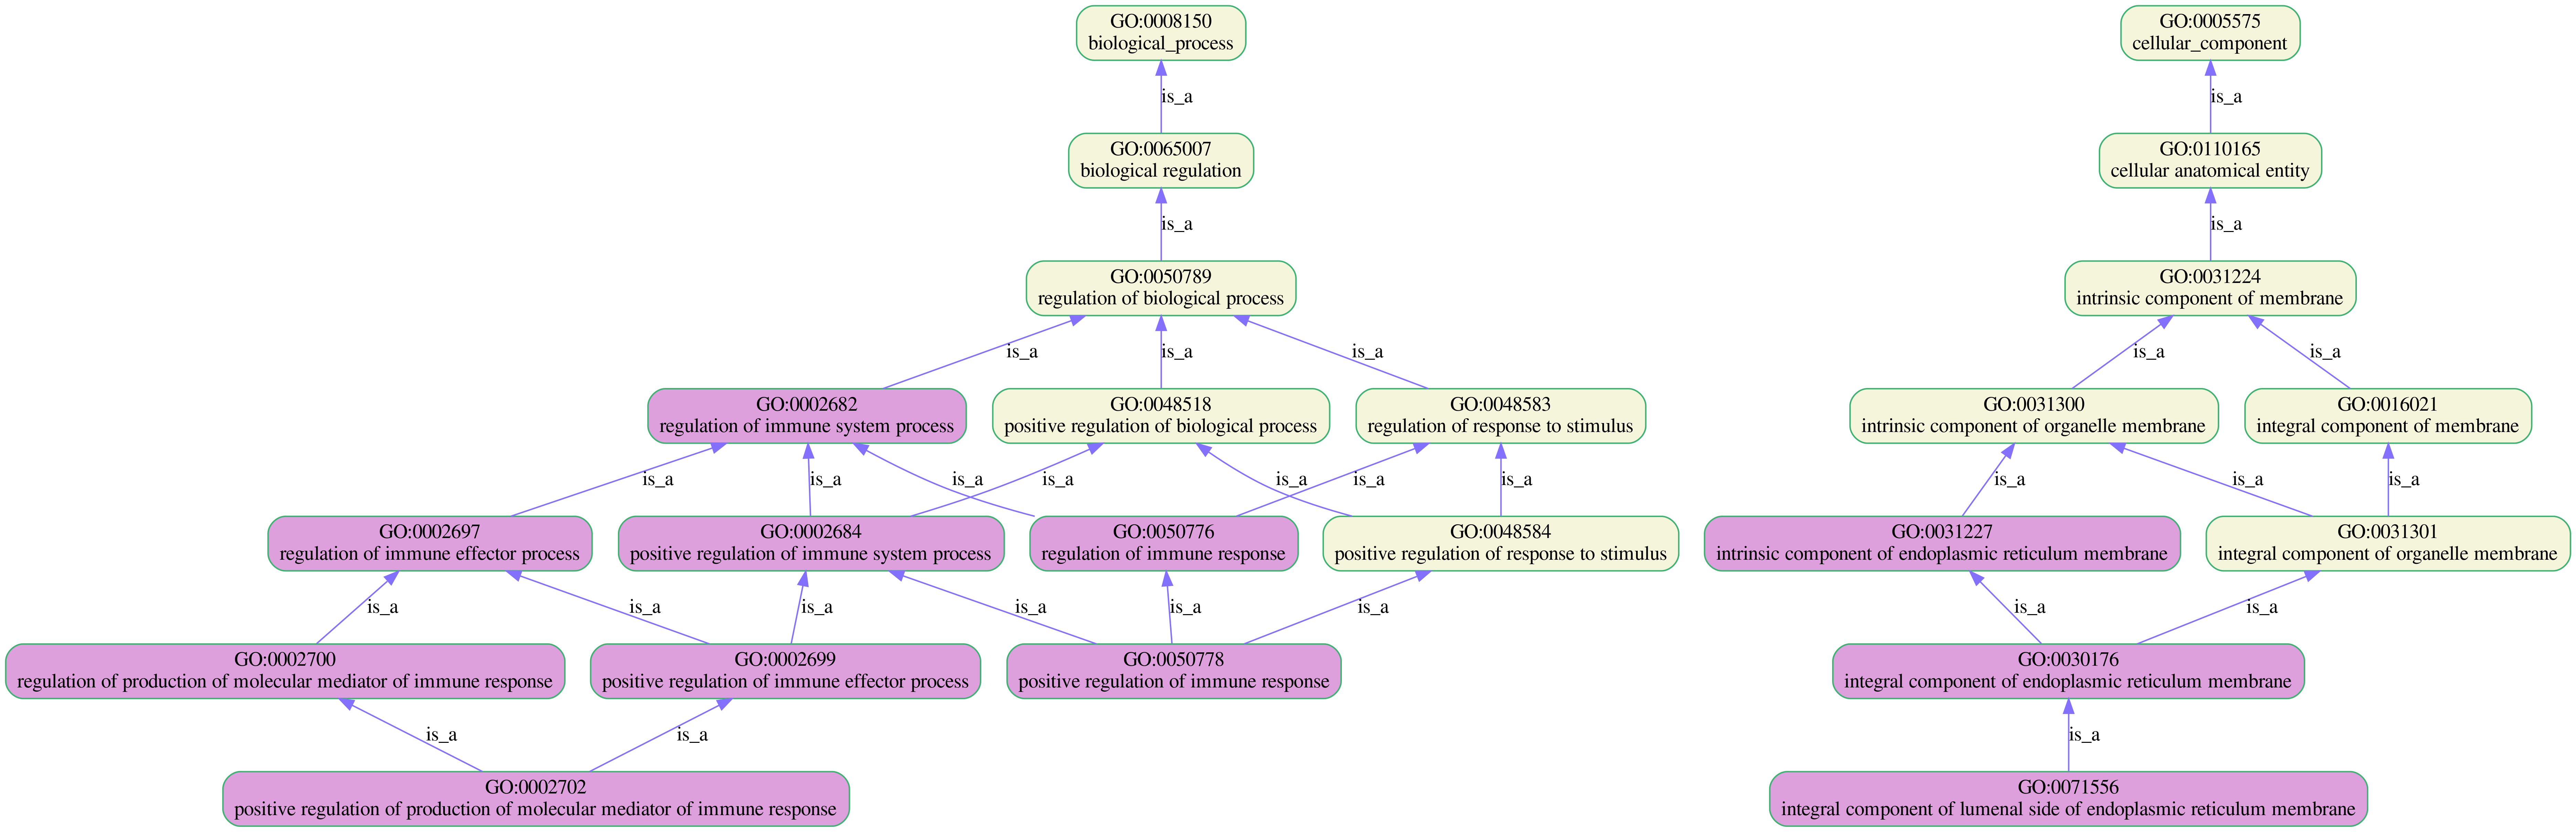
\includegraphics[scale=0.07]{\plotspath{TCGA_OV_VST/GeneEnrichment/go_lineage_5_of_ICA_5.png}} \\
\begin{spacing}{0.6}
{\small Genes: \tiny \input{/home/ipoole/Documents/gitrepos/HgsocTromics/Plots/TCGA_OV_VST/GeneEnrichment/go_gene_set_5_of_ICA_5.txt}}
\end{spacing}
\vspace{0.5cm}
{\small Component ICA-5-of-5} \\
\caption{Lineage maps of enriched Gene Ongology (GO) terms for components ICA-3-of-5 and ICA-5-of-5}
\label{fig-ICA-3-5-go-lineage}
\end{center}
\end{figure}


\begin{sidewaysfigure}[ht]
\begin{center}
\includegraphics[width=\textwidth]{\plotspath{TCGA_OV_VST/GeneEnrichment/go_lineage_4_of_ICA_5.png}} \\
\begin{spacing}{0.6}
{\small Genes: \tiny \input{/home/ipoole/Documents/gitrepos/HgsocTromics/Plots/TCGA_OV_VST/GeneEnrichment/go_gene_set_4_of_ICA_5.txt}}
\end{spacing}
\vspace{0.5cm}
\caption{Lineage maps of enriched Gene Ongology (GO) terms for component ICA-4-of-5. For this component it was necessary to additionally filter the enriched terms -- see text.}
\label{fig-ICA-4-go-lineage}
\end{center}
\end{sidewaysfigure}


\begin{figure}[ht]
\begin{center}
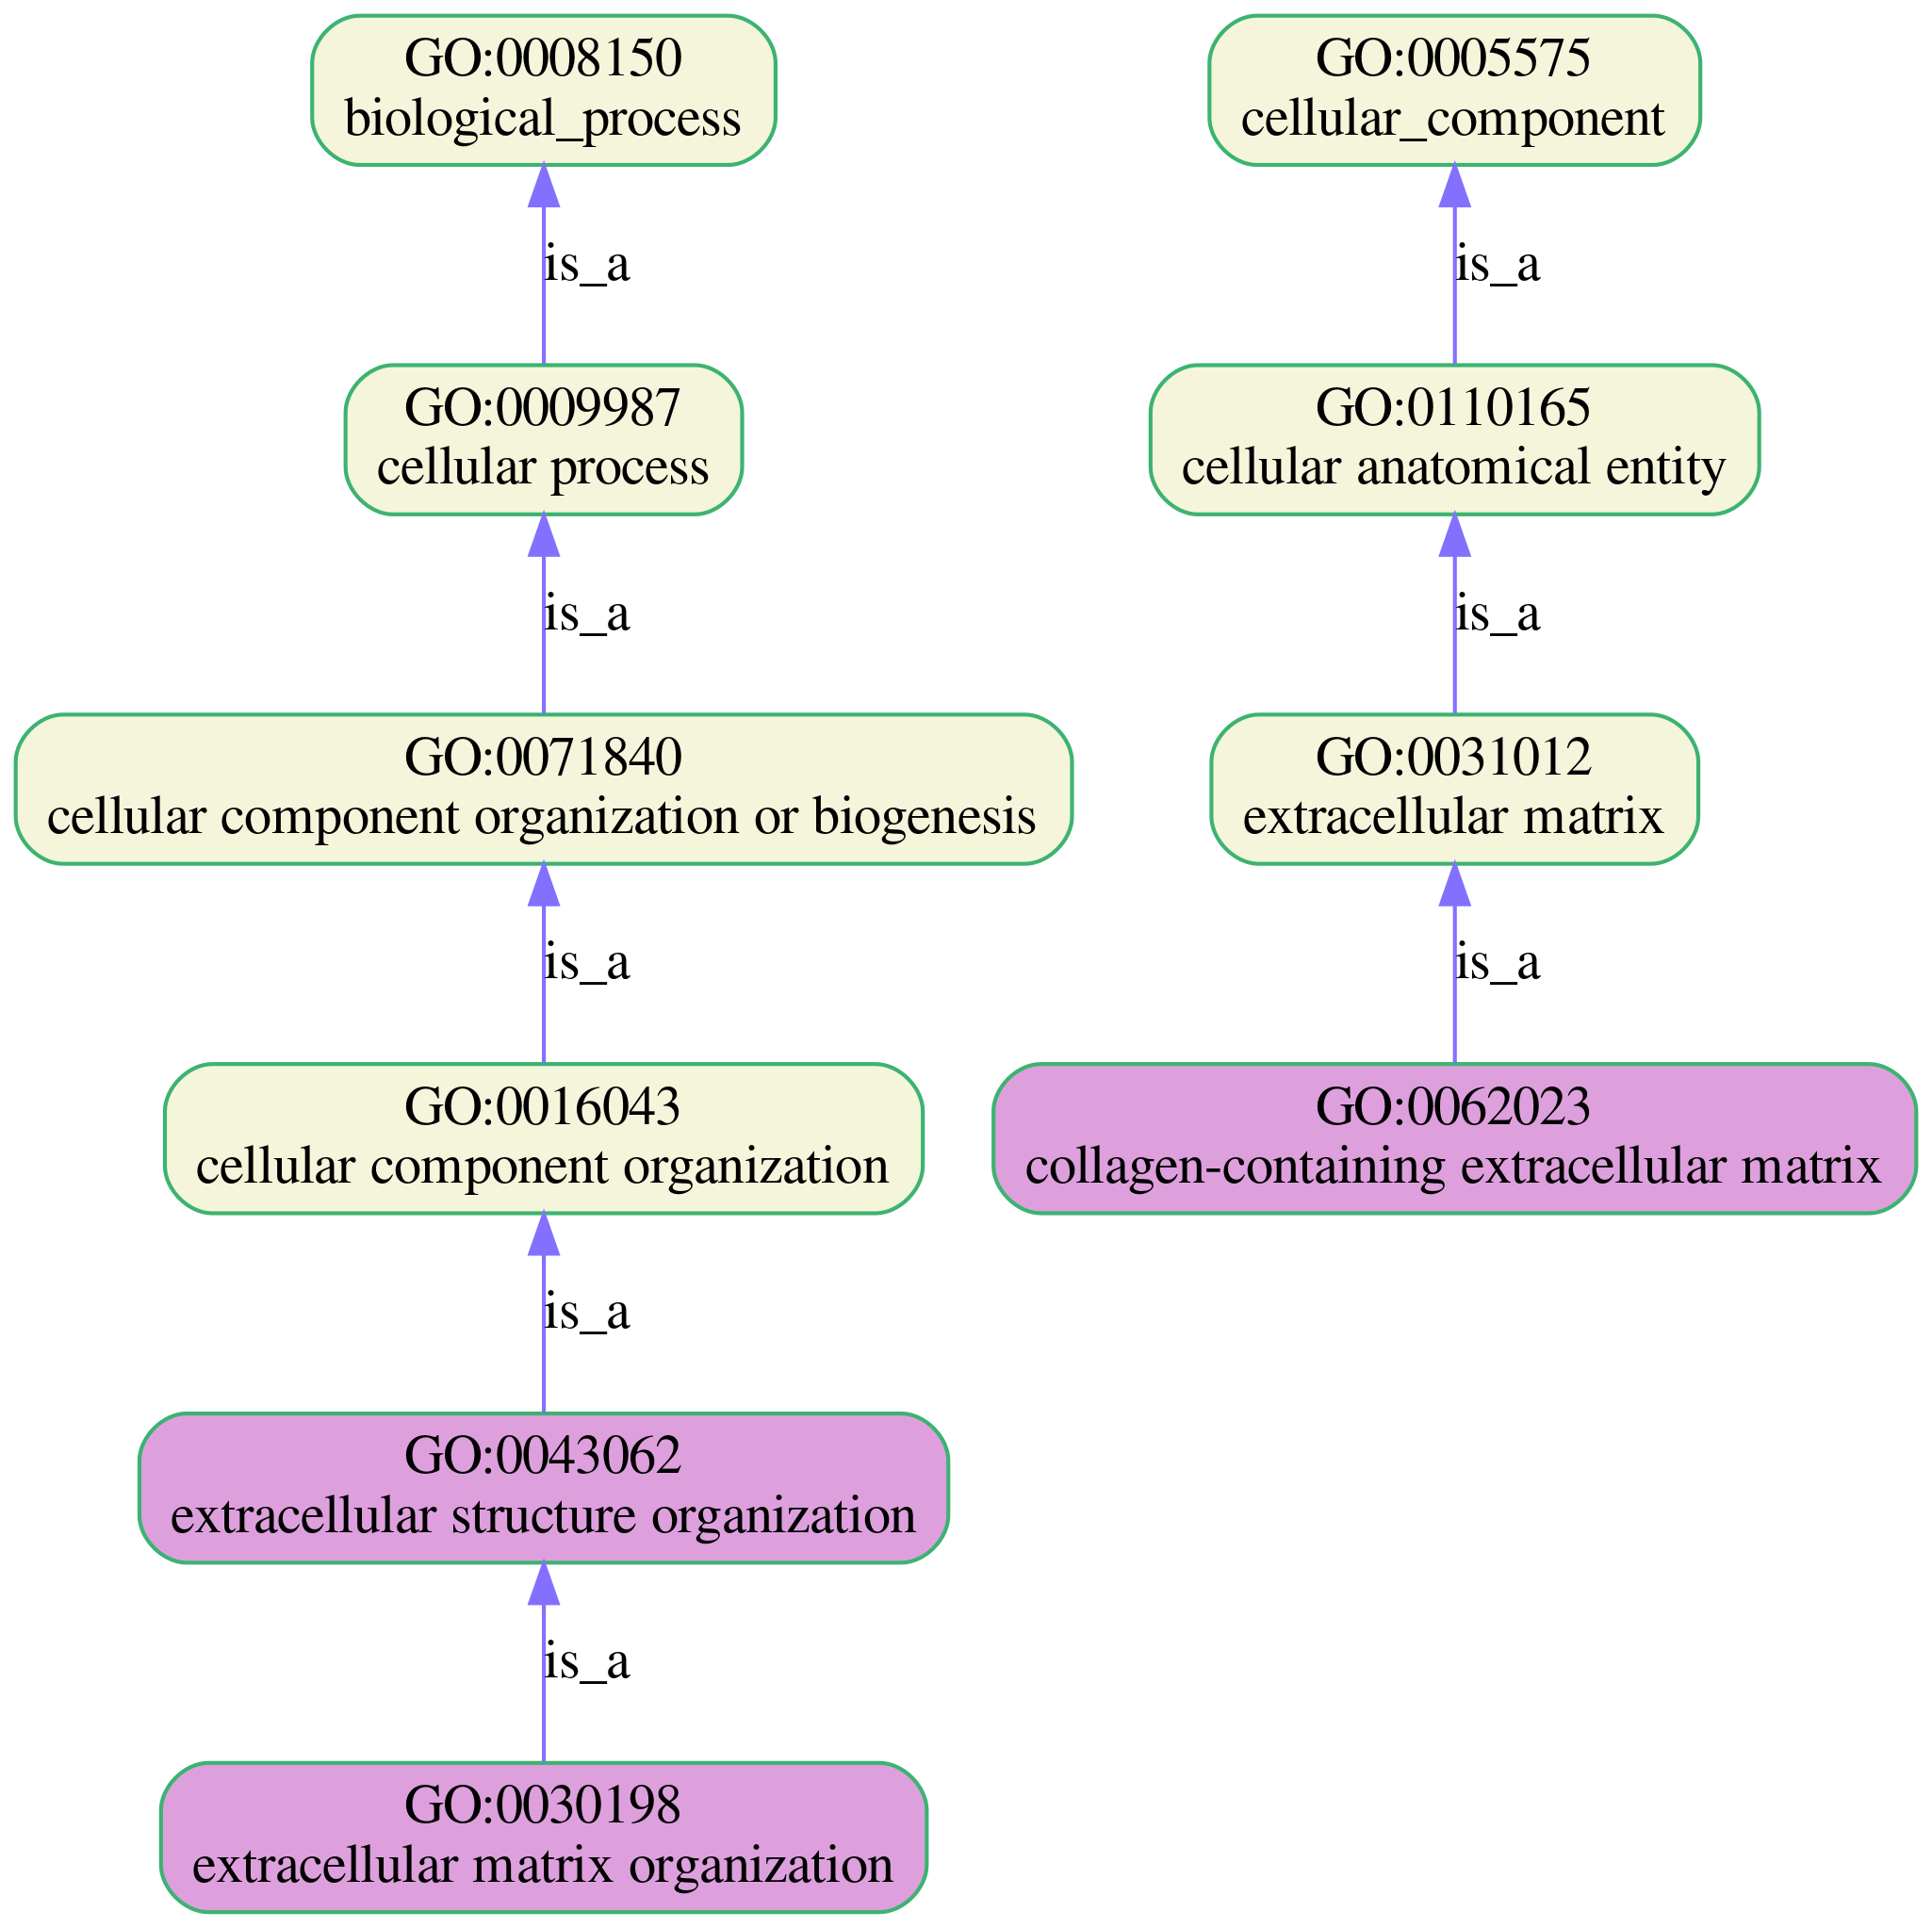
\includegraphics[width=0.5 \textwidth]{\plotspath{TCGA_OV_VST/GeneEnrichment/go_lineage_1_of_PCA_3.png}} \\
\begin{spacing}{0.6}
{\small Genes: \tiny \input{/home/ipoole/Documents/gitrepos/HgsocTromics/Plots/TCGA_OV_VST/GeneEnrichment/go_gene_set_1_of_PCA_3.txt}}
\end{spacing}
\vspace{0.5cm}
{\small Component PCA-1-of-3} \\
\vspace{1cm}
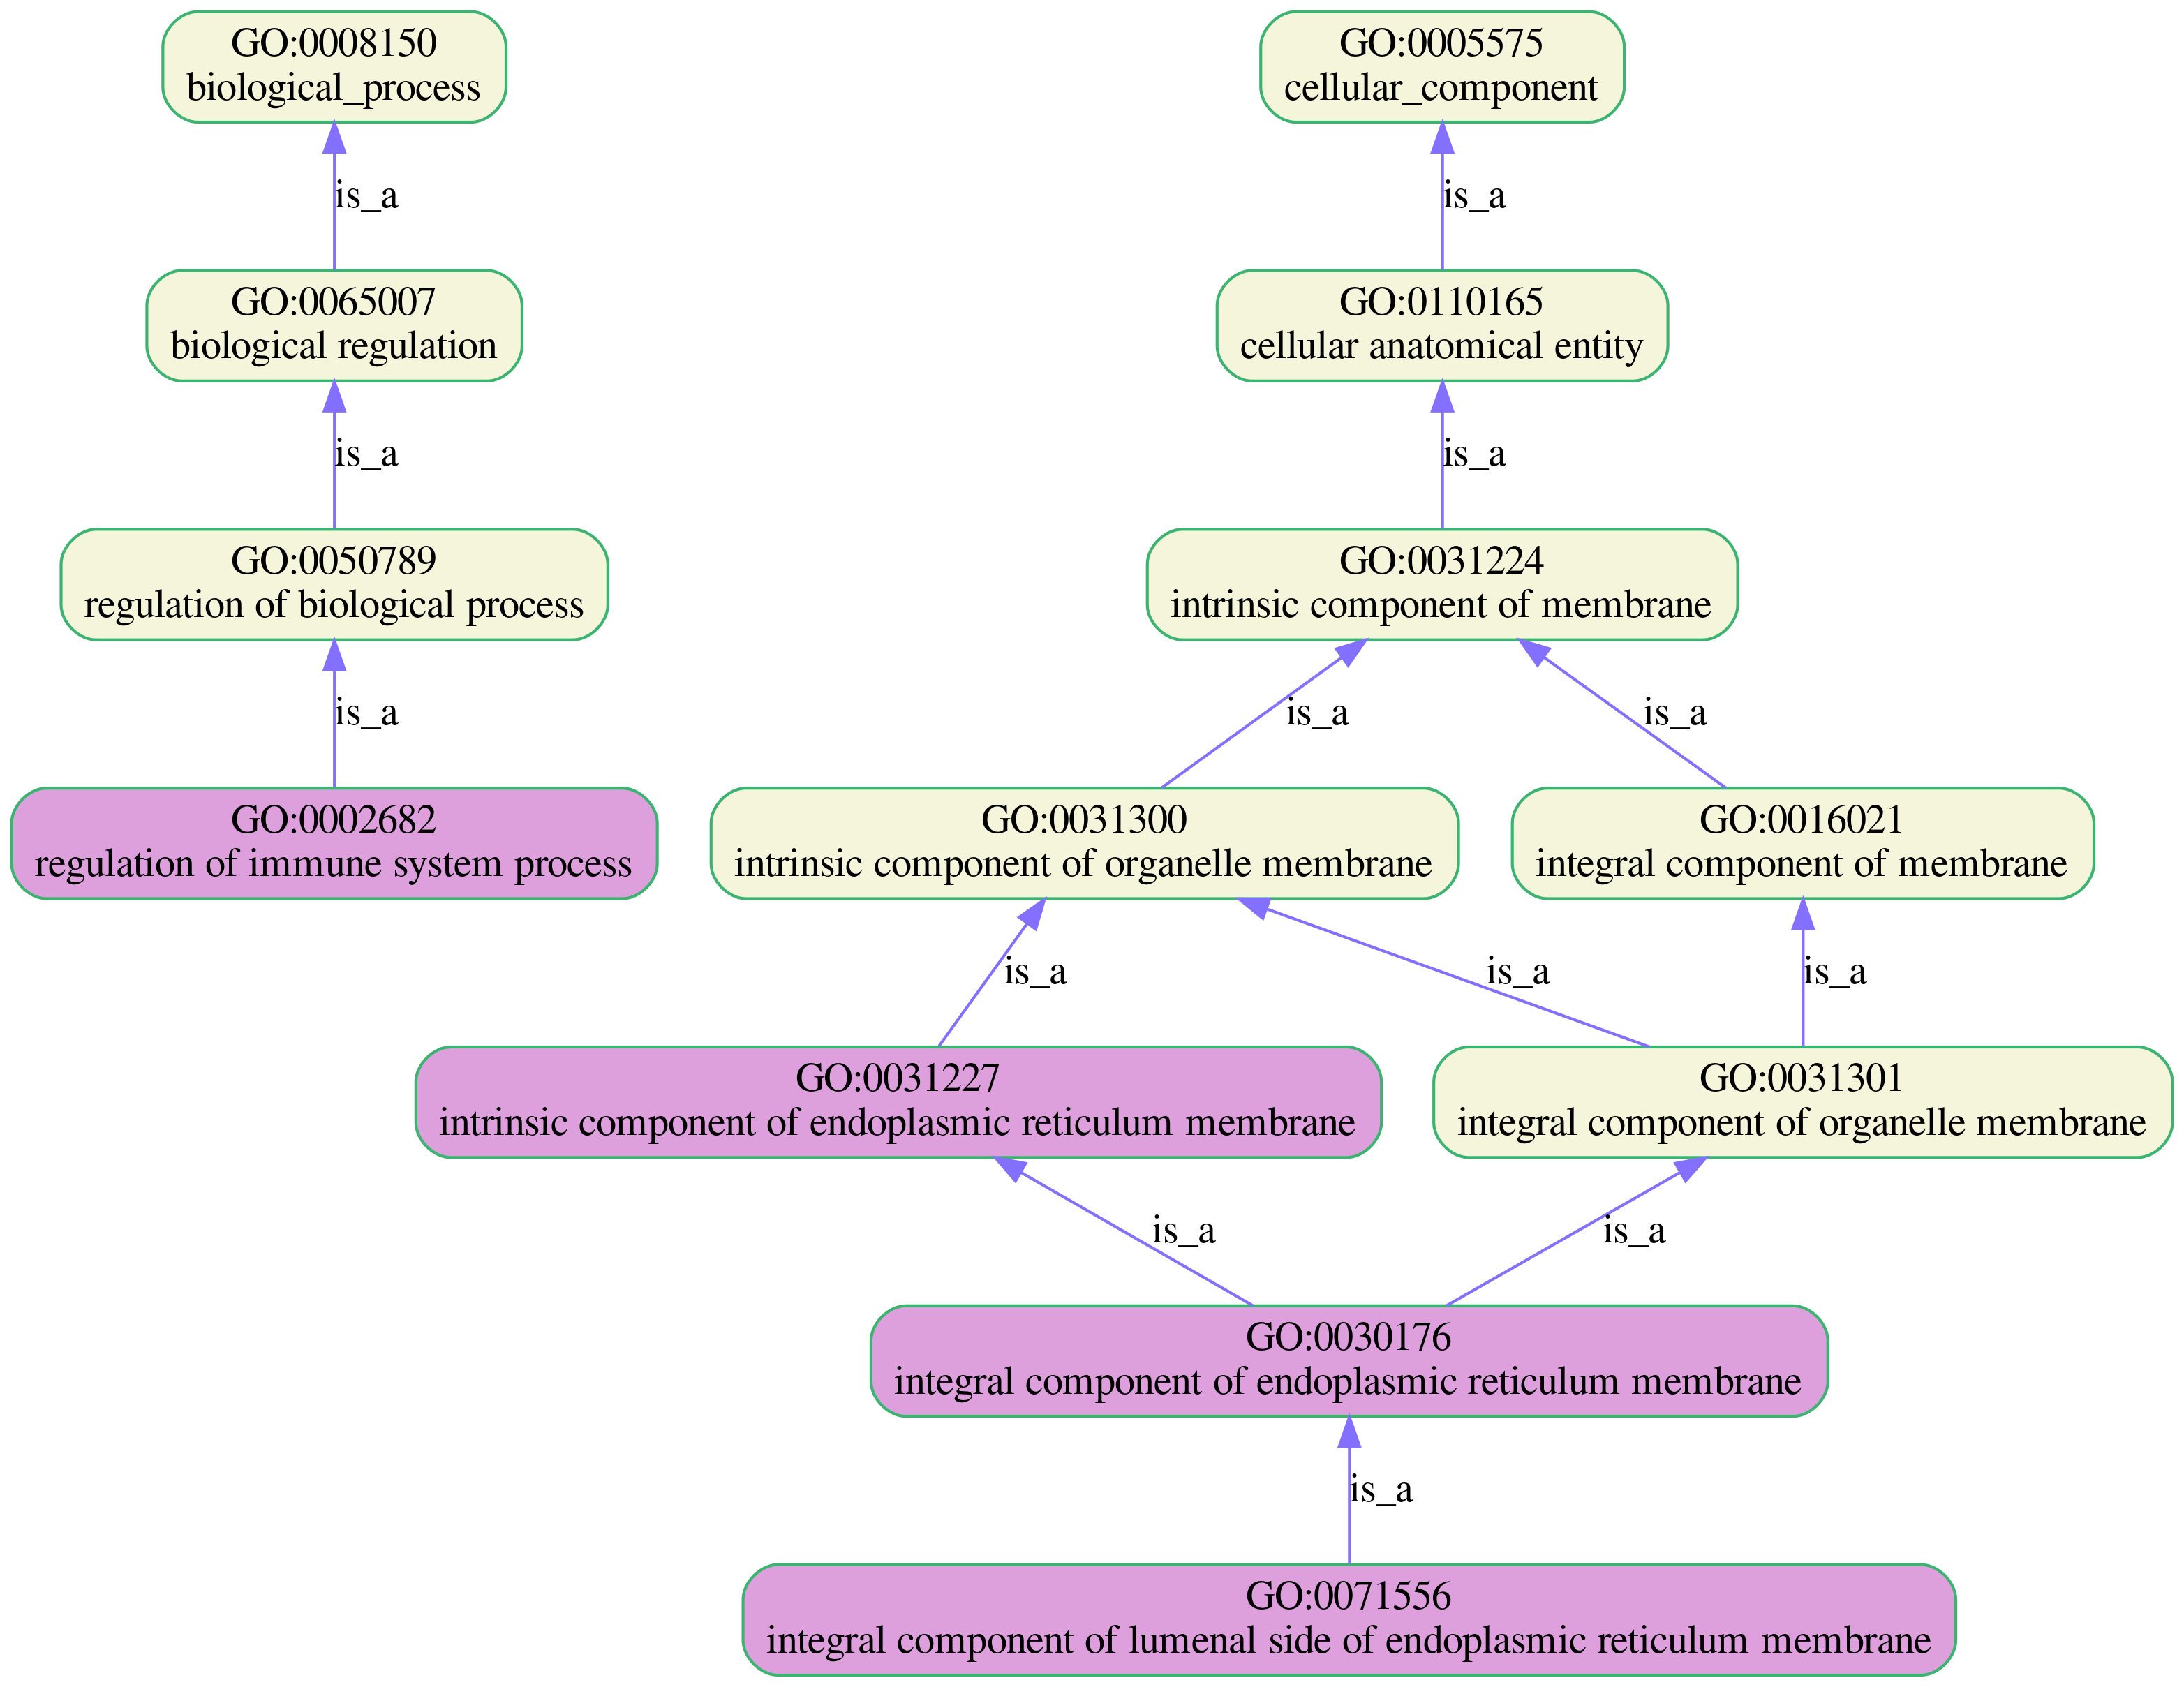
\includegraphics[width= \textwidth]{\plotspath{TCGA_OV_VST/GeneEnrichment/go_lineage_3_of_PCA_3.png}} \\
\begin{spacing}{0.6}
{\small Genes: \tiny \input{/home/ipoole/Documents/gitrepos/HgsocTromics/Plots/TCGA_OV_VST/GeneEnrichment/go_gene_set_3_of_PCA_3.txt}}
\end{spacing}
\vspace{0.5cm}
{\small Component PCA-3-of-3} \\
\caption{Lineage maps of enriched Gene Ongology (GO) terms for components 1 and 3 from the rank=5 PCA factorization. (Component PCA-2-of-3 produced no significant enrichment results)  }
\label{fig-PCA-1-3-go-lineage}
\end{center}
\end{figure}

Considering the biological significance of each of the 11 extracted metagenes, with reference to the GO enrichment results:
\begin{description}
%
\item[NMF 1-of-3]: this is related to the cellular structures and processes of the extra-cellular matrix (ECM), that is the proteins such as collagens which mediate the three-dimensional organisation of cells in a tissues.  ECM molecular composition will vary substantially between tissue types, but is also known to play a part in many disease processes \cite{Theocharis2019}.  Thus, this metagene may simply reflect heterogeneity of tissues in the biopsied sample, or may have some deeper disease related significance.
%
\item[NMF 2-of-3]: here we see enrichment of genes relating to the ribosomal subunit and the processes of RNA binding, implying perhaps a link with assembly of the ribosomal RNA-protein complex.   Ribosomes are known to have a role in carcinogenesis, by dysregulation the RNA $\rightarrow$ protein translation, or mutations in ribosomal subunits impacting on cellular metabolism \cite{Sulima2017}.
%
\item[NMF 3-of-3, ICA 1-of-5 and ICA 2-of-5]: no significant biological enrichment found.
%
\item[ICA 3-of-5]: this component relates to processes of multicellular / extracellular organisation, and the ECM.  It is therefore similar to NMF 1-of-3 above.
\item[ICA 4-of-5]: this component is seen to relate to the ribosomal subunit (as NMF 2-of-3), additionally membrane proteins in the respiratory complex, mitochondrial and the NADH dehydrogenase complex.  Processes of organonitrogen biosynthesis are also highlighted. 
%
\item[ICA 5-of-5]: processes relating to regulation of immune response are enriched in this component, featuring genes from the major histocompatibility complex group, in particular the HLA- genes, allowing the immune system to recognise self from non-self.  GO terms relating to the endoplasmic reticulum (ER) are also highlighted.  It may be that this component is mainly sensitive to the immunohistochemical signature of patients, and therefore not of clinical interest.
%
\item[PCA 1-of-3]: there is mention of ECM related terms, as for ICA 3-of-5 and NMF 1-of-3.   However, there are also terms relating to the regulation of angiogenesis.  It is known that tumours have a need for increased blood supply, and that expression level of factors promoting angigenesis are associated with aggresiveness of tumour growth \cite{Nishida2006}.  
We have already seen (section \ref{sec-subtype-classification}, \cite{Glass2015}) there is evidence for distinct subtypes of OC distinguished by angiogenesis related genes, and that these subtypes have been found to inform clinical outcome \cite{Glass2015}.  Thus, this component might contain useful prognostic value.
%
\item[PCA 2-of-3]: no significant biological enrichment found.
%
\item[PCA 3-of-3]: this component has some similarity with ICA 5-of-5, in that it refers to regulation of immune processes (HLA- genes) and ER membrane.   However, chemotaxis (cell movement) is also highlighted.
\end{description}

We have noted above that both NMF 1-of-3 and ICA 3-of-5 may be related to tissue type heterogeneity.  We have also seen from metasample heatmap analysis that these two metagenes are associated with closely correlated metasamples (in AOCS), and also to have a moderately high Jaccard similarity of 0.39.  Further, we observed that these components correlate negatively with cellularity.  This is as one would expect: low cellularity implies a mixture of tumour and non-tumour cell types, resulting in variation of ECM composition. 

Interestingly, the above summary of the gene enrichment results tentatively suggests component PCA 1-of-3 is most likely to have clinical prognostic value, based on a cursory look at the literature.  This perhaps supports an earlier observation that, while not conclusive, component PCA-1-of-3 comes closest to demonstrating correlation with patient survival (section \ref{sec-survival-analysis}, figure \ref{fig-summary-survival-plots}).

How should we interpret those four components which demonstrate no significant enrichment with biological meaning?  It is notable that all three methods have at least one such component.  Among these four, PCA 1-of-3 and ICA 1-of-5 have high (the highest) Jaccard similarity of 0.61.   For all other pairs among these four Jaccard similarity is negligible.  Perhaps these two components are picking up on similar technical variation between the samples?   


\clearpage

\subsection{Association of unsupervised gene expression patterns with patient survival is inconclusive}

Kaplan-Meier overall survival (OS) plots stratified by each metasample component are shown for the TCGA dataset in figure \ref{fig-kaplan-meier-os-TCGA-TCGA} and for the AOCS dataset in figure \ref{fig-kaplan-meier-os-TCGA-AOCS}.  Plots for progression free survival (PFS) on AOCS can be found in the appendix, figure \ref{fig-kaplan-meier-pfs-TCGA-AOCS}.   All plots show 95\% confidence intervals and hazard ratio (HR) with associated p-value.

All of these results are summarised in figure \ref{fig-summary-survival-plots}, which brings together the three sets of results -- TCGA (OS), AOCS (OS) and AOCS (PFS) --  with respect to the 11 metasample components.  $\log_2{\mbox{HR}}$ is used in order that the \emph{sense} of the survival impact can be readily appreciated.    If a metasample component has a robust correlation with survival, then we expect the p-value for all three sets of results to show significance \emph{and} for the effects to have the same sense -- be in the same direction.  None of the 11 components pass this test.   

The component with the largest observed effect on survival is PCA 1-of-3, showing a reasonably consistent hazard ratio of around 1.3 ($2^{0.4}$) across the three experiments.  This has $p < 0.05$ in the larger TCGA dataset, but not in the smaller AOCS dataset.

\begin{figure}[ht]
\begin{center}
\includegraphics[scale=0.5]{\plotspath{SurvivalAnalysis/multiple_kaplan_meier_os_TCGA_TCGA.pdf}} 
\caption{Kaplan-Meier plots for each metasample component, stratified at the median value, for TCGA $\rightarrow$ TCGA for overall survival (OS) case.  Hazard ratio and p-value is shown for each case.  The final plot (bottom right) is unstratified overall survival}
\label{fig-kaplan-meier-os-TCGA-TCGA}
\end{center}
\end{figure}


\begin{figure}[ht]
\begin{center}
\includegraphics[scale=0.5]{\plotspath{SurvivalAnalysis/multiple_kaplan_meier_os_TCGA_AOCS.pdf}} 
\caption{Kaplan-Meier plots for TCGA $\rightarrow$ TCGA for overall survival (OS).}
\label{fig-kaplan-meier-os-TCGA-AOCS}
\end{center}
\end{figure}


\begin{figure}[ht]
\begin{center}
\includegraphics[scale=0.5]{\plotspath{/SurvivalAnalysis/survival_summary_barplots_NMF.pdf}} \\
\includegraphics[scale=0.5]{\plotspath{/SurvivalAnalysis/survival_summary_barplots_ICA.pdf}} \\
\includegraphics[scale=0.5]{\plotspath{/SurvivalAnalysis/survival_summary_barplots_PCA.pdf}}
\caption{Visual summary of survival analysis as applied to TCGA(OS), AOCS(OS) and AOCS(PFS).  Plots are divided by factorization method.  Bar heights show $\log_2(\mbox{HR})$ with p-value also shown.}
\label{fig-summary-survival-plots}
\end{center}
\end{figure}

\clearpage


%The dendrogram clustering of metasamples (columns, top of figures) gives insights into the similarity of each metasample component, while the clustering of patients (rows, left of figures) offers insights into sub-populations of patients and how (in the case of AOCS only) these relate to metadata variables such as cellularity and mutational load.   
%These topics will be taken up in the following discussion section.


\subsection{Metasample correlation with genomic features}

From the grid of scatter plots shown in figure \ref{fig-genomic-scatters} it can be seen there are some significant correlations.  
The sense (sign) of the correlation is arbitrary -- particularly for ICA and PCA -- recall normalisation w.r.t $180^\circ$ was applied. 
 
The significant correlations are summarised in table \ref{tab-genomic-scatter-summary}.  
WGD and Cellularity show correlation with at least one component from all three methods and indeed three components correlating with WGD also correlate with Cellularity and in the same sense.  
This might suggest simply that WGD and Cellularity are themselves correlated, but this is not so: $r=-0.14, p=0.201$ for Point-Biserial correlation (data not shown).  % Latent factor??
HR Detect correlates with two NMF and one ICA component, not intersecting with those above, suggesting distinct biological processes are involved.

The heatmap dendrogram (figure \ref{fig-heatmap-TCGA-AOCS}) shows close correlation between metasamples pairs (NMF-1-of-3, ICA-5-of-5), (ICA-1-of-5, PCA-2-of-3) and (NMF-1-of-3, ICA-3-of-5).

\begin{figure}[ht]
\begin{center}
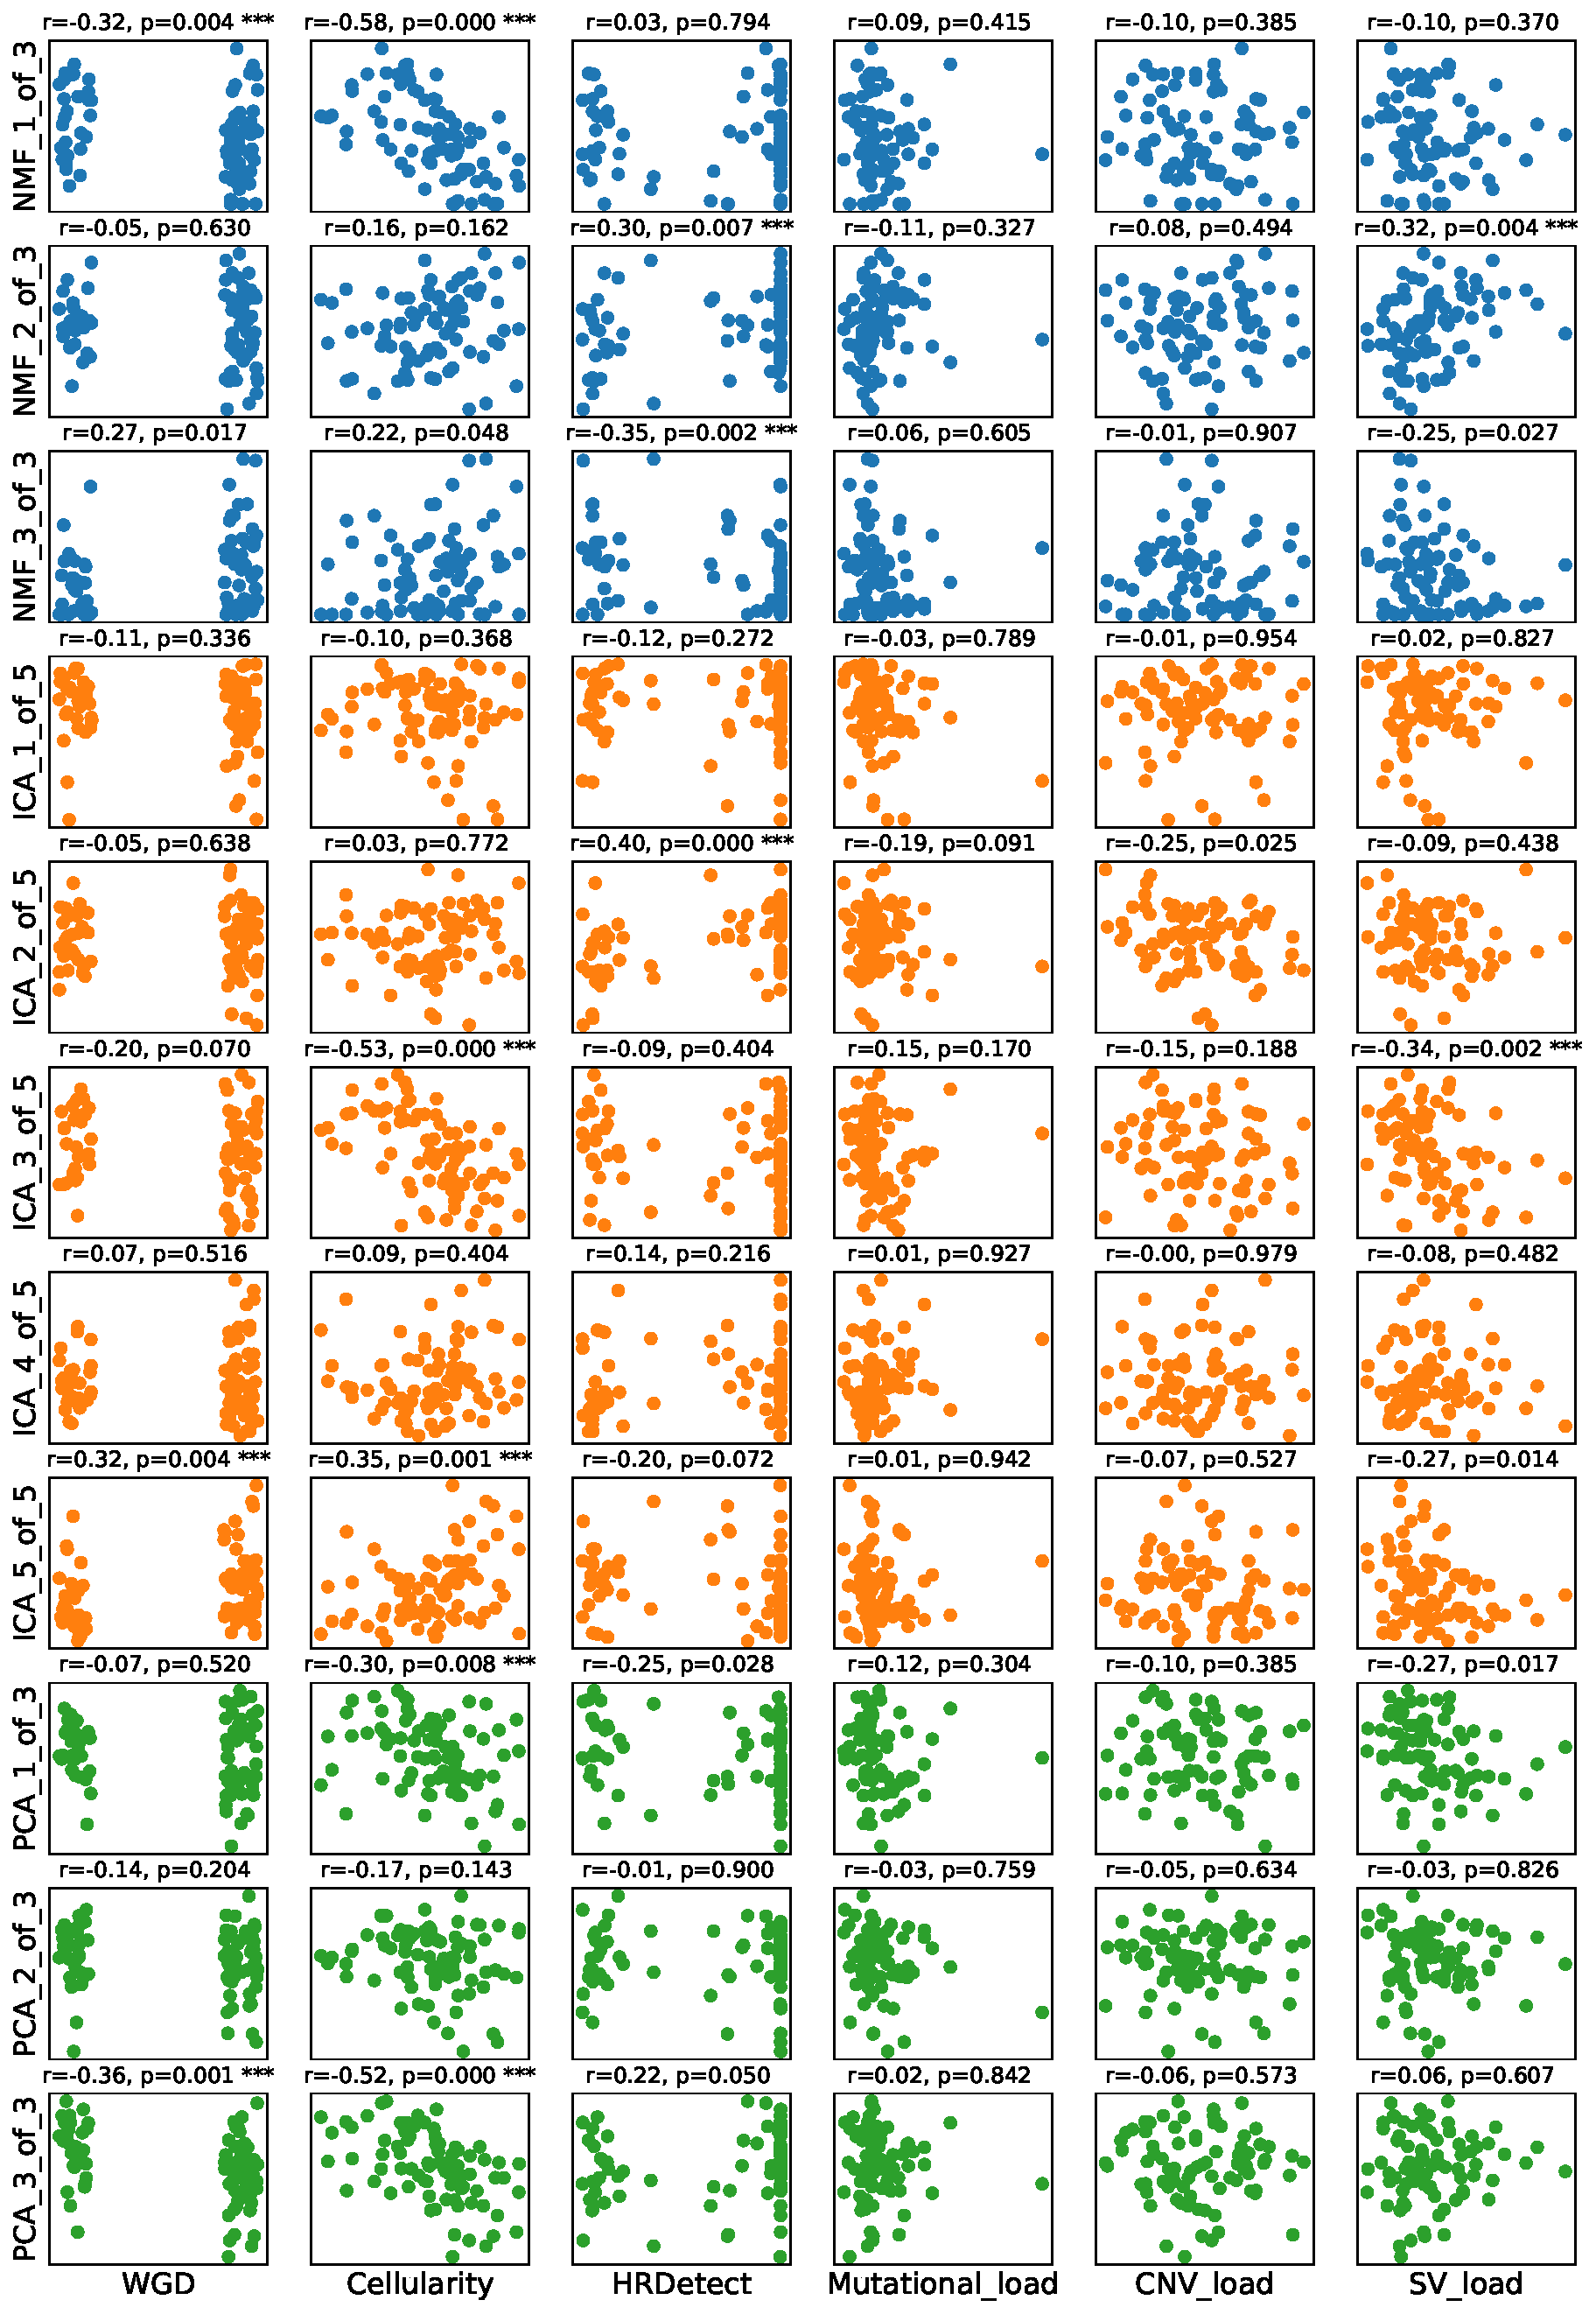
\includegraphics[scale=0.5,draft=false]{\plotspath{BoxAndScatters/genomic_feature_scatters_TCGA_AOCS.pdf}} 
\caption{Grid of scatter plots to visualise the correlation between metasamples and genomic features.  In the case of WGD which has binary values (0, 1), jitter is applied for visual effect only.   Above each plot is shown a correlation coefficient $r$ and associated p-value, highlighted with '***' where $p < 0.01$.  In the case of WGD , the Point-Biserial correlation is used; for all others Pearson's $r$ is used.}
\label{fig-genomic-scatters}
\end{center}
\end{figure}

\begin{figure}[ht]
\begin{center}
\includegraphics[scale=0.7, draft=false]{\plotspath{HeatMaps/clustered_heatmap_TCGA_AOCS.pdf}} 
\caption{Heatmap of the metasamples matrix for the AOCS dataset, computed from metagenes factorized from the TCGA dataset.   Several patient metadata variables are shown in columns to the left.}
\label{fig-heatmap-TCGA-AOCS}
\end{center}
\end{figure}

\begin{table}[ht]
\begin{center}
\begin{tabular}{|l|l|}
\hline
Genomic feature & Significant correlations \\
\hline 
WGD & NMF-1-of-3, ICA-5-of-5, PCA-3-of-3 \\
Cellularity & NMF-1-of-3, ICA-3-of-5, ICA-5-of-5, PCA-3-of-3 \\
HR Detect & NMF-2-of-3, NMF-3-of-3, ICA-2-of-5 \\
Mutational load & None \\
CNV load & None \\
SV load & NMF-2-of-3 \\
\hline
\end{tabular}
\end{center}
\caption{Summary of metasample components showing a significant correlation with each genomic feature.}
\label{tab-genomic-scatter-summary}
\end{table}

\clearpage

\section{Discussion}

One valuable lesson from this work is the importance of accounting for sampling error, by bootstrapping,  when considering the stability of factorizations and thence the selection of factorization rank.    Sevaral authors comment on the variability of NMF and ICA factorization due to algorithm initialisation \cite{Kairov2017,Sompairac2019,WayGregory2019}, but most neglect sampling error which we have shown to be far more significant.   Cantini \etal\ \cite{Cantini2019a} mention bootstrapping, in reference to the BIODICA package (for ICA factorization), but it is unclear whether this is applied to the input data to model sampling error.  In the initial stages of the current work, BIODICA was used, and was found to recommend ranks of 14, 19 or 30.  Yet we have seen that such high ranks on the small n=80 dataset leads to highly unstable factorizations when bootstrap modelling of sampling error is included.

These considerations lead to the selection of much lower ranks (fewer metagenes) than would otherwise be the case.

\emph{TODO: much more discussion!}


\subsection{Further work}

This work has thrown up several possible lines of further study:
\begin{enumerate}
\item
{\bf Algorithm hyper-parameters}.  NMF and ICA algorithms have a number of hyper-parameters, only a few of which were explored in this work.  For example, NMF has parameters to encourage sparsity through L1 regularization.   This should result in many (most?) metagene elements reducing to zero, and might offer a more robust means of selecting candidate genes to feed into gene enrichment analysis -- replacing the current arbitrary 3 SD from the mean rule.
\item
{\bf Discovering batch effects}.  It has been claimed (e.g. \cite{Stein-OBrien2018}) that matrix factorization methods are an effective means of identifying and removing batch effects.  This could be explored by horizontally concatenating the TCGA and AOCS datasets (after gene set intersection), producing an $n=80+274=354$ dataset with a substantial batch artefact.  Factorizations of this combined dataset should be more robust because of the larger $n$.  Does each of NMF, ICA and PCA naturally produce a component which correlates with batch?
\item
{\bf Selecting components from several factorization ranks}.
In the current work, a single rank was selected for each method -- 3, 5 an 3 for NMF, ICA and PCA respectively.  Unlike PCA, components extracted by NMF and ICA  do not `nest' with rank; that is adding rank in general yields a new set of components.  Thus one might, for NMF and ICA, perform factorizations at $k=2,3,4,5$, say, yielding $2 \times 15 = 30$ potential components in total.  Jaccard similarity could be used to identify that subset of components which had the least overlap in detected genes.   In this way, a larger number of components could be obtained without use of high factorization ranks which we have seen to be unstable.
\item
{\bf Cross-dataset factorization stability}.  We went to considerable effort -- through bootstrap sampling and cluster analysis -- to select factorization ranks which we hoped would be robust and generalise well to other datasets.   A way to confirm this robustness would be to perform the factorization / clustering pipeline on \emph{both} datasets separately, yielding two sets of metagenes.  In a perfect world, these metagenes would pair up identically (in-so-far as the two datasets had identical technical characteristics, drawn from identical population of patients).  The Jaccard similarity heatmap could be used to verify this, and reject components which showed low cross-dataset similarity.
\item
{\bf Contrasting gene expression patterns between cancers}.  The current work set out to find patters of gene expression in HGSOC.  Yet it is hard to say the highlighted patterns are specific to HGSOC, or generic to all cancers.  One way of teasing out cancer specific patterns might be to take a similar approach to the previous item, but instead of looking for metagenes which are consistent between datasets, find those which are distinct.  That said, there will likely be many more sophisticated approached in the literature, given the clinical importance of the topic.
\item
{\bf Systematic comparison with published gene expression patterns}.  In analysing the meaning of each metagene above, some tentative links were made with the research literature.   But this was anecdotal and frankly not particularly scientific; searching on PubMed for GO terms associated with HGSOC and looking at one or two hits!  A more systematic and ideally automated approach is required.  The \href{https://www.ncbi.nlm.nih.gov/geoprofiles}{Geo Profiles database} at NCBI, or the \href{https://www.ebi.ac.uk/gxa/home}{Expression Atlas} at EMBL-BI might be possible starting points.

\end{enumerate}


\section{Conclusions}
TODO

\bibliography{OvarianCancer}
\bibliographystyle{ieeetr}

\section{Appendices}
\subsection{Additional figures and plots}

\begin{figure}[ht]
\begin{center}
\includegraphics[scale=\S]{\plotspath{AOCS_Protein/FactorClustering/multiple_single_factors_scatter_AOCS_NMF_2_3_5_10_fixed.pdf}} \\
\includegraphics[scale=\S]{\plotspath{AOCS_Protein/FactorClustering/multiple_single_factors_scatter_AOCS_NMF_2_3_5_10_bootstrap.pdf}}\\
\caption{Clustering of metagenes from NMF facorizations on the AOCS dataset, comparing fixed and bootstrap sampling}
\label{fig-AOCS-nmf-fixed-vs-bootstrap}
\end{center}
\end{figure}

\begin{figure}[ht]
\begin{center}
\includegraphics[scale=\S]{\plotspath{AOCS_Protein/FactorClustering/multiple_single_factors_scatter_AOCS_PCA_2_3_5_10_fixed.pdf}} \\
\includegraphics[scale=\S]{\plotspath{AOCS_Protein/FactorClustering/multiple_single_factors_scatter_AOCS_PCA_2_3_5_10_bootstrap.pdf}}\\
\caption{Clustering of metagenes from PCA facorizations on the AOCS dataset, comparing fixed and bootstrap sampling}
\label{fig-AOCS-pca-fixed-vs-bootstrap}
\end{center}
\end{figure}


\begin{figure}[ht]
\begin{center}
\includegraphics[scale=0.5]{\plotspath{SurvivalAnalysis/multiple_kaplan_meier_pfs_TCGA_AOCS.pdf}} 
\caption{Kaplan-Meier plots for TCGA $\rightarrow$ TCGA for progression free survival (PFS).  }
\label{fig-kaplan-meier-pfs-TCGA-AOCS}
\end{center}
\end{figure}


TODO - I'll likely move the AOCS survivial plots here, and perhaps some of the GO lineages.
\begin{figure}[ht]
\begin{center}
\includegraphics[scale=0.6]{\plotspath{BoxAndScatters/wgd_boxplot_NMF_TCGA_AOCS.pdf}}
\includegraphics[scale=0.6]{\plotspath{BoxAndScatters/wgd_boxplot_ICA_TCGA_AOCS.pdf}}
\includegraphics[scale=0.6]{\plotspath{BoxAndScatters/wgd_boxplot_PCA_TCGA_AOCS.pdf}}
\caption{Boxplots showing relationship between metasamples (derived from TCGA metagenes, applied to AOCS data) and whole genome doubling (WGD) status.  Metasamples from NMF, ICA and PCA are shown separately.  To allow convenient visualisation, each metasample is normalised to zero mean unit variance, hence between metasample variation is removed.}
\end{center}
\label{fig-wgd-boxplots}
\end{figure}


\subsection{Gene enrichment raw results}
\label{tab-go-enrichment-results}
TODO
\subsection{Software libraries and versions}
TODO
\label{sec-software-versions}


\end{document}
